\chapter{Prototyp}
\label{sec:Prot:first}

Dieses Kapitel beschäftigt sich mit der Planung, dem Aufbau und einer Evaluierung zweier Smart-Building-Prototypen mit LoRaWAN. 

\section{Problemstellung}
\label{sec:Prot:problem}

Selbst wenn man sich nur auf LoRaWAN als IoT-Protokoll beschränkt, sind die Möglichkeiten, ein Smart Building IoT-Netzwerk aufzubauen, unzählig. Neben Netzwerkprovidern, wie beispielsweise Loriot oder aufeinander abgestimmten Komponenten von The Things Industries und dem The Things Stack, existiert eine Vielzahl an Open-Source-Lösungen. Zudem besteht eine IoT-Lösung nicht nur aus dem Netzwerk, über das die Daten versandt werden, sondern einer Datenverwaltung und einer Möglichkeit diese Daten zu visualisieren. Auch hier sind die Auswahlmöglichkeiten nahezu endlos. In dieser Arbeit wird daher ein exemplarischer Prototyp mit möglichst vielen, extern bereitgestellten Services, unter anderem einem öffentlichen LoRaWAN-Netzwerk, und ein zweiter Prototyp mit ausschließlich Open-Source-Software und einem eigenen, privaten Netzwerk, erstellt. Es soll zum Schluss eine begründete Aussage getroffen werden können, welche der Möglichkeiten, beziehungsweise welche Kombination der genutzten Tools, für welche Zwecke am besten geeignet ist.

\section{Verwendete Geräte}
\label{sec:Prot:hardware}

Um ein realistisches Smart Building Szenario mit dem Prototypen nachzustellen, wurden als LoRaWAN-Endgeräte pro Prototyp jeweils ein Temperatur- und Luftfeuchtigkeitssensor (LHT65) und ein Türsensor (LDS01) von der chinesischen Firma Dragino genutzt. Die beiden Sensoren werden in Abbildung \ref{fig:sensors} gezeigt. Der Temperatursensor sendet hierbei alle 20 Minuten eine Nachricht mit drei Messwerten über Temperatur und Luftfeuchtigkeit und weitere Metainformationen wie dem Lade\-stand des Akkus und kostet derzeit in etwa 30€ pro Stück. Der Türsensor hingegen sendet alle 24 Stunden und bei jeder Öffnung und Schließung der Tür eine Nachricht mit dem aktuell Türzustand, der gesamten Anzahl an Türöffnungen, der letzten Öffnungsdauer und ebenfalls Metainformationen wie den Akkustand und ist mit etwa 15€ Stückpreis ebenfalls sehr günstig zu haben. Der ursprüngliche Plan, die Sensoren selbst zu bauen, wurde schnell verworfen, da es nur schwer möglich ist, die Akkulaufzeit und vor allem den Preis der gewählten käuflichen Sensoren zu schlagen.

\begin{figure}[H]
  \vspace{10pt}
  \begin{center}
    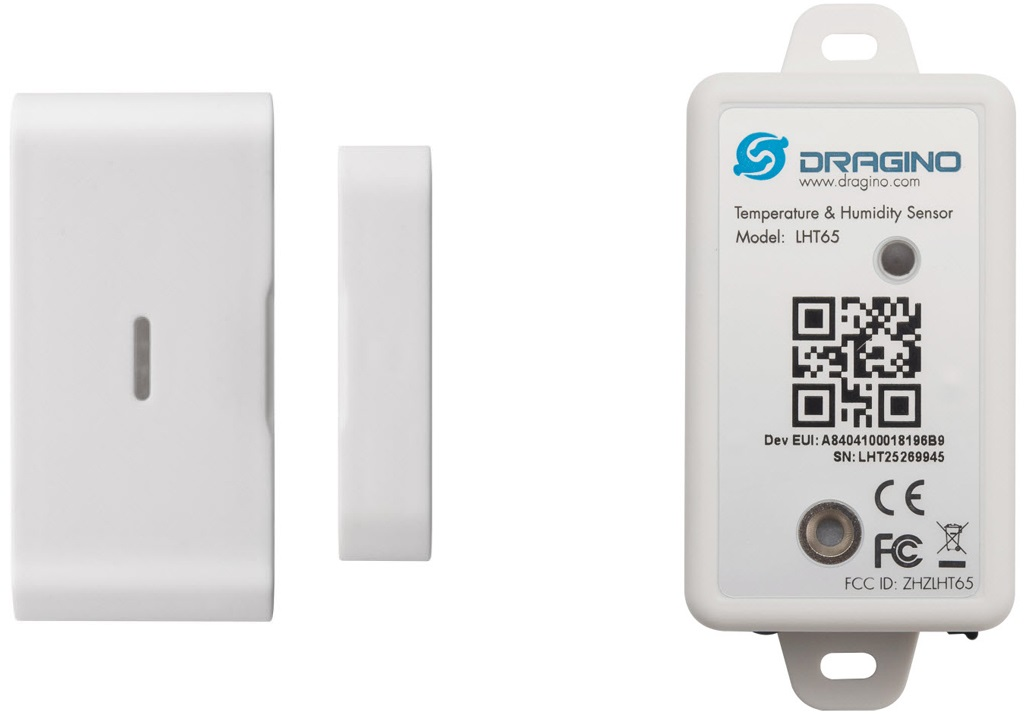
\includegraphics[width=0.6\textwidth]{./images/sensoren.jpg}
  \end{center}
  \vspace{-5pt}
  \caption[Dragino LDS01 und Dragino LHT65 Sensoren]{Dragino LDS01 (links) und Dragino LHT65 (rechts)}
  \caption*{Quelle: {dragino.com/products/products-list.html (bearbeitet)}}
  \label{fig:sensors}
\end{figure}

Auch LoRa-Empfangsstationen gehören zur Hardware hinzu. Für den ersten Prototypen wurde ein offizielles Gateway von The Things Industries verwendet, da derartige Gateways wie in Kapitel \ref{sec:ThHi:ttntti}  beschrieben bereits für das The Things Network vorkonfiguriert sind, und somit die Inbetriebnahme deutlich vereinfachen. Das hier verwendete Gateway ist mit einem Preis von etwa 300€ zwar sehr teuer, es existieren jedoch mittlerweile deutlich günstigere Gateways für das The Things Network. Für den zweiten Prototypen wurde das LPS8 Indoor Gateway von der Firma Dragino genutzt. Dieses Gateway ist für etwa 100€ erhältlich. Abbildung \ref{fig:gateways} zeigt die beiden verwendeten Gateways.

\begin{figure}[H]
  \vspace{10pt}
  \begin{center}
    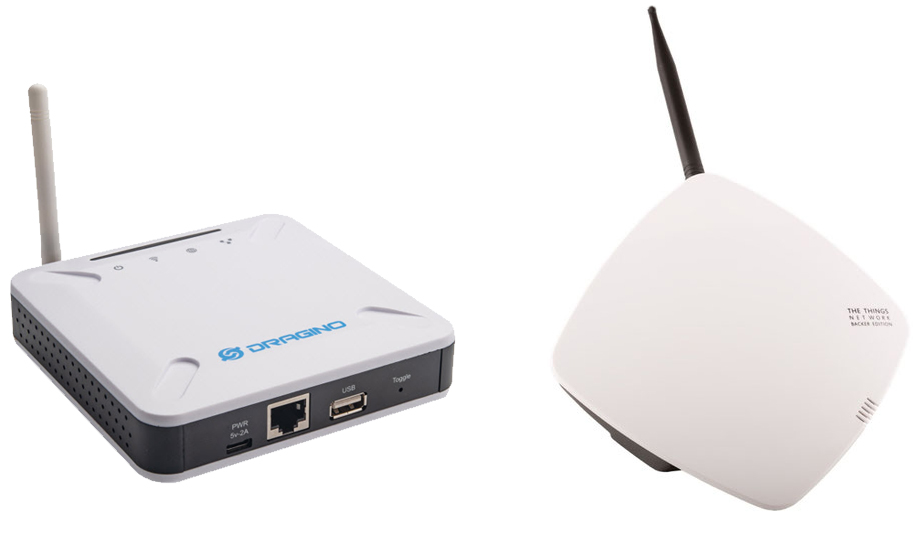
\includegraphics[width=0.85\textwidth]{./images/gateways.jpg}
  \end{center}
  \vspace{-5pt}
  \caption[Dragino LPS8 Gateway und The Things Gateway]{Dragino LPS8 (links) und The Things Gateway}
  \caption*{Quelle 1: {dragino.com/products/lora-lorawan-gateway/item/148-lps8.html (bearbeitet)}}
  \vspace{-10pt}
  \caption*{Quelle 2: {daizy.io/product/the-things-gateway (bearbeitet)}}
  \label{fig:gateways}
\end{figure}

% https://www.dragino.com/media/k2/galleries/148/LPS8-10.jpg
% https://daizy.io/product/the-things-gateway/

\section{Time-Series-Datenbanken}
\label{sec:Prot:timeseriesdb}

Eine wichtige Architekturentscheidung in jedem Softwareprojekt ist die Auswahl einer Datenbank zur Datenverwaltung, so auch in IoT-Projekten. Während im Bereich der Softwareentwicklung der Trend immer mehr in die Richtung der NoSQL-Datenbanken geht, rückt im Bereich des Internet of Things ein neuer Kandidat ins Rampenlicht: Time-Series-Datenbanken. Um dies zu verstehen, gilt es zuerst zu betrachten, wie die Datenverwaltung von IoT-Daten funktioniert. Da meist Daten von vielen verschiedenen Sensoren erhoben werden, diese jedoch nur sporadisch eingesehen werden, ist die Anzahl der Schreiboperationen um ein Vielfaches höher als die der Leseoperationen. Zudem ist für Messwerte immer der Zeitpunkt der Messung interessant, um später zeitabhängige Trends in den Daten erkennen zu können. Unter diesem Aspekt ensteht auch der Name der Datenbanken: es handelt sich um Time-Series-Data, also eine nach der Zeit sortierte Datensequenz wie zum Beispiel den Verlauf der Raumtemperatur eines Gebäudes. 

Allein anhand der Datenstruktur kann die Beliebtheit von Time-Series-Datenbanken im IoT-Bereich leicht erklärt werden. In typischen, relationalen Datenbanken werden Daten in verschiedenen Tabellen mit verschiedenen Verknüpfungen, sogenannten Relationen, gespeichert. Außerdem sind diese Datenbanken primär für Lesezugriffe optimiert. Ein Problem hierbei ist die Struktur der Daten selbst: in relationalen Datenbanken kann pro Tabelle nur ein Schema, also eine Datenstruktur, hinterlegt werden. Somit müssten in großen Projekten unzählige Tabellen erstellt werden.
Da IoT-Daten außerdem meist keinerlei Relationen benötigen und wie bereits erwähnt meist deutlich mehr Schreiboperationen als Lesezugriffe verursachen, sind rela\-tionale Datenbanken nicht perfekt für diesen Usecase geeignet.\\ Genau hier kommen Time-Series-Datenbanken ins Spiel, indem sie genau diese Probleme lösen. Die Datenbanken sind dafür optimiert, viele Schreiboperationen in kurzer Zeit zu tolerieren. Meist werden die Daten in einer Key-Value Struktur hinterlegt, wobei der Key einen Timestamp darstellt. Somit sind gespeicherte Daten nicht nur automatisch zeitlich sortiert, sondern weisen außerdem eine flexible Datenstruktur auf. Der Value kann verschiedenste Werte enthalten und somit Daten von verschiedensten Geräten speichern, ohne mehrere Datenbankinstanzen oder Tabellen zu benötigen. Dies resultiert zwar in einem Mehraufwand bei Datenänderungen, jedoch ist es eher untypisch IoT-Daten wie Messwerte manuell zu verändern.\\ 
Ein weiteres Feature vieler Time-Series-Datenbanken beschäftigt sich mit den Daten selbst. Daten können nach einer bestimmten Lebenszeit automatisch gelöscht werden (Data Lifecycle Management / Retention Policy) oder in bestimmten Zeitblöcken zusammengefasst (Data Summarization) werden. Dies ist interessant, da in IoT-Daten wie zum Beispiel dem Temperaturverlauf eines Gebäudes zwar eine hohe Präzision der letzten Stunden oder Tage, nicht aber der letzten Monate oder Jahre erwünscht ist. Je nach Einstellung könnte also die Datenbank zum Beispiel Daten die älter sind als einen Monat von einem Datenpunkt pro Sekunde zu einem Datenpunkt pro Tag zusammenfassen, wodurch pro Tag nur noch etwa 0.0012\% des vorherigen Speichers verbraucht werden. Diese Präzision reicht jedoch meist völlig aus, um beispielsweise Langzeittrends in den Daten zu erkennen. Eine derartige Logik müsste bei der Nutzung einer normalen relationalen Datenbank aufwendig auf Softwareseite gelöst werden und ist daher meist nicht praktikabel. Nicht zuletzt durch diese Techniken, aber auch durch weitere Optimierungen ist es mit Time-Series-Datenbanken möglich, Abfragen über Millionen von Datenpunkten in wenigen Millisekunden auszuführen. Aus diesen Gründen gehören diese Datenbanken zu den beliebtesten im IoT-Bereich und werden auch hier in beiden Prototypen gewählt. Mehr Informationen über Time-Series-Datenbanken und deren Anwendungsmöglichkeiten können in den Artikeln \cite{TimeSeriesWater.2019} und \cite{TimeSeriesInflux.2020} nachgelesen werden.

\clearpage

\section{Prototyp 1: The Things Network mit Azure IoT Central}
\label{sec:Prot:version1}

Der erste Prototyp wurde unter der Nutzung von möglichst vielen, extern angebotenen Services und Hardwarekomponenten, erstellt. In diesem Kapitel werden eine Beispielarchitektur sowie Erfahrungen und Ergebnisse des Prototyps vorgestellt. Die beiden großen Softwarekomponenten sind hierbei LoRaWAN-seitig das \Fachbegriff{The Things Network} und \Fachbegriff{Microsoft Azure IoT Central} für alle weiteren Funktionen.

\subsection{Erwartungen}
\label{sec:Prot:erwartungen1}

Da in dem Aufbau des Prototypen primär vorkonfigurierte, teilweise sogar kostenpflichtige Services genutzt werden, können klare Erwartungen sowohl an den Aufbau als auch an die Ergebnisse selbst gestellt werden. Die wohl größte Erwartung liegt in der Natur der Cloudservices: es ist nicht nötig, Server selbst aufzusetzen und zu konfigurieren. Auch der LoRaWAN-Stack besteht aus vorkonfigurierten und interoperablen Softwarekomponenten, wie bereits näher in Kapitel \ref{sec:ThHi:ttntti} erklärt wurde. Da außerdem Gateways von \Fachbegriff{The Things Industries} genutzt werden, sollte das Setup der gesamten IoT-Lösung allgemein sehr einfach und kaum zeitaufwendig sein. Eine weitere Erwartung ist eine gute Skalierbarkeit des Systems und vor allem das einfache Hinzufügen neuer Geräte ohne aufwendige Konfiguration. Eine zu diesem Zeitpunkt noch unbehandelte Frage ist die Datenverbindung zwischen dem The Things Network und Azure IoT Central, die im Kapitel \ref{sec:Prot:systemkomponenten1} geklärt wird. Sind die Daten erst einmal in Azure IoT Central, wird eine Vielzahl an nützlichen Features erwartet, um die IoT-Daten zu speichern, zu verwalten oder live zu überwachen. Außerdem soll eine Nutzer- und Rechteverwaltung des Netzwerks möglich sein.

\subsection{Systemkomponenten}
\label{sec:Prot:systemkomponenten1}

Wie bereits erwähnt wird als LoRaWAN-Stack das The Things Network genutzt. Für diesen kleinen Prototypen reicht die Community Edition, also das kostenlose Nutzen des öffentlichen Netzwerks völlig aus. Für sehr große Deployments bietet es sich jedoch an über The Things Industries eine Individuallösung zu beantragen. Zur Verwaltung der Daten wird Azure IoT Central verwendet. Es handelt sich hierbei um die 2018 erschienene IoT-Plattform von Microsoft. Die Entwickler geben an, dass es mit der Plattform möglich sein soll, beliebig große, skalier\-bare und sichere IoT-Anwendungen zu erschaffen, ohne selbst ein Verständnis beziehungsweise Kenntnisse der Cloud zu benötigen. Besonders nützlich ist jedoch die Integration in andere Microsoft Services. So kann beispielsweise auf Sensordaten reagiert werden, indem mit Tools wie Microsoft Flow oder Azure Functions automatisierte Vorgänge ausgeführt werden. Auch Datenvisualisierung mit dem erprobten Tool \Fachbegriff{PowerBI} ist durch diese Integration möglich. Allgemein versucht Azure IoT Central die Komplexität aus IoT-Lösungen zu nehmen und somit das Einrichten einer solchen Lösung zu erleichtern \Zitat{IoTCentral.2019}.

\subsection{Umsetzung}
\label{sec:Prot:umsetzung1}

Die Aufsetzung des ersten Prototypen begann mit der Aktivierung der Endgeräte. Nachdem ein Account im The Things Network angelegt ist, können, wie in Kapitel \ref{sec:ThHi:ttntti} beschrieben, Applications in der sogenannten ``The Things Network Console'', einer Art Kommandozentrale für das eigene Netzwerk, erstellt werden, mit denen später hinzugefügte Geräte assoziiert werden können. Die Aktivierung selbst funktioniert sehr einfach über OTAA oder ABP, wobei in diesem Fall OTAA gewählt wurde. Hierfür muss zuerst die AppEUI in der aktuellen Application hinterlegt werden. Nun kann das Gerät mithilfe eines in der Application eindeutigen Namens, der DevEUI und dem AppKey dem Netzwerk hinzugefügt werden. Sendet das Endgerät nun eine Nachricht, die von einem beliebigen Gateway des The Things Network empfangen wird, erreicht die Nachricht die eigene Application. Betrachtet man die Nachricht, fällt jedoch auf, dass das gesendete Payload hexadezimal dargestellt wird. Dies liegt daran, dass LoRaWAN-Nachrichten meist binär enkodiert werden, um die Nachrichtengröße zu reduzieren und somit mehr Nachrichten pro Tag senden zu können. Um den wahren Inhalt des Payloads zu lesen, kann im The Things Network pro Application eine sogenannte \Fachbegriff{Decoder-Funktion} erstellt werden. Nutzt man selbstgebaute Endgeräte, muss das Enkodieren und Dekodieren selbst programmiert werden, während bei käuflichen Endgeräten die Decoder-Funktion meist mitgeliefert wird. Die gesamte Verwaltung kann durch Rollen und Rechte an verschiedene Nutzer verteilt werden und ist somit selbst für die Zusammenarbeit vieler Personen geeignet.

Nun wird eine Azure IoT Central Anwendung erstellt. Wie bereits angesprochen, muss ein Weg geschaffen werden, Daten aus dem The Things Network in die Azure IoT Central Anwendung weiterzuleiten. Die Lösung hierfür scheint etwas komplizierter als erwartet, jedoch existiert zum aktuellen Zeitpunkt keine einfachere Möglichkeit. Microsoft Azure veröffentlichte für derartige Vorhaben die ``iotc-device-bridge'' als Open-Source-Projekt auf GitHub\footnote{\url{github.com/Azure/iotc-device-bridge}}, welche es Nutzern ermöglicht, Daten aus anderen IoT-Cloud-Services an Azure IoT Central zu senden. Das Funktionsprinzip selbst ist hierbei recht einfach. Die Device Bridge wird als Azure Function, also als eine Azure Ressource bereitgestellt. Bei Azure Functions handelt es sich um eine Möglichkeit, Programmcode beim Aufkommen verschiedenster Events auszuführen, ohne dafür einen Server aufsetzen zu müssen. So ist es beispielsweise möglich, HTTP-basierte Endpunkte mit Azure Functions zu verwirklichen \Zitat{AzureFunction.2016}. Genau dieser Funktionalität macht sich die Device Bridge zunutze. Die Applikation empfängt Nachrichten via HTTP vom The Things Network und leitet diese durch die Azure Infrastruktur an die IoT Central Application weiter. Viele IoT-Cloud-Services, wie auch der Application Server des The Things Network bieten sogenannte Integrations an. Integrations sind Möglichkeiten, Daten aus dem The Things Network an andere Dienste weiterzuleiten. Naheliegend war in der Erstellung dieses Prototypen die Nutzung der HTTP Integration, die eingehende Nachrichten an einen HTTP-Endpoint weiterleiten kann. Somit musste lediglich die Azure Device Bridge als HTTP-Endpoint für diese Integration konfiguriert werden. Nun finden die Daten ihren Weg von den LoRaWAN-Endgeräten bis hin zur IoT Central Anwendung.

Um eingehende Daten in Azure IoT Central nutzen zu können, müssen vorerst sogenannte ``Device Templates'' erstellt werden. Diese stellen ein semantisches Mapping der Rohdaten auf eine virtuelle Kopie des genutzten Gerätes dar. Hier werden alle vorhandenen Werte und deren Einheiten strukturiert festgelegt. Dies bietet den großen Vorteil, dass Nutzer bei der Einsicht der Daten kein genaues Verständnis über die Daten benötigen und keine Rohdaten interpretieren müssen. Sendet ein Gerät zum ersten Mal eine Nachricht, muss das Gerät manuell in IoT Central einem Device Template zugeordnet werden. Von diesem Zeitpunkt an können die Daten sinnvoll genutzt werden. Das Hinzufügen neuer Geräte funktioniert also ohne aufwendige Konfiguration und erfordert lediglich das Registrieren des Geräts im The Things Network und die Zuweisung zu einem Device Template in Azure IoT Central.

\begin{figure}[H]
  \vspace{10pt}
  \begin{center}
    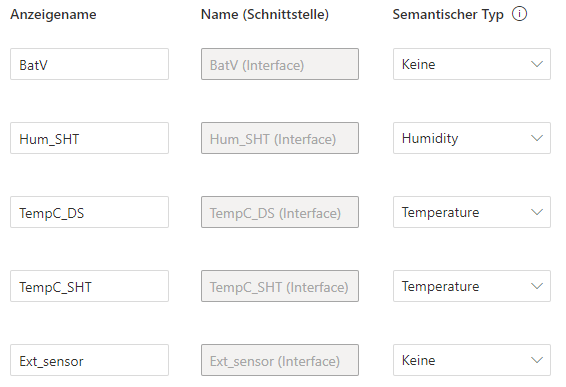
\includegraphics[width=0.8\textwidth]{./images/device-template.png}  
    \end{center}
  \vspace{-5pt}
  \caption[IoT Central Device Template]{IoT Central Device Template}
  \label{fig:device-template}
  \vspace{-10pt}
\end{figure}

Abbildung \ref{fig:device-template} zeigt das Device Template des im Prototypen genutzten Temperatursensors. Es fällt auf, dass beispielsweise dem Attribut ``TempC\_DS'', also einem Temperaturwert, der semantische Typ ``Temperature'' zugeordnet ist. Somit muss der Wert von Endnutzern nicht mehr als numerischer Wert interpretiert werden.

Die wohl einfachste Nutzung der Daten ist die Visualisierung. Hierfür können ganze Dashboards zusammengestellt werden, in denen die Daten durch verschiedene Graphen oder Ansichten dargestellt werden. Das Erstellen solcher Visualisierungen ist hier sehr einfach, da IoT Central durch die Device Templates bereits versteht, welche Visualisierungen für die jeweilige Datenstruktur möglich ist. So ist beispielsweise ein Graph für Temperaturdaten sehr geeignet, während für ein Protokoll aus Zuständen wie Türöffnungen eher eine textuelle Liste sinnvoll ist. 

\begin{figure}[H]
  \vspace{10pt}
  \begin{center}
    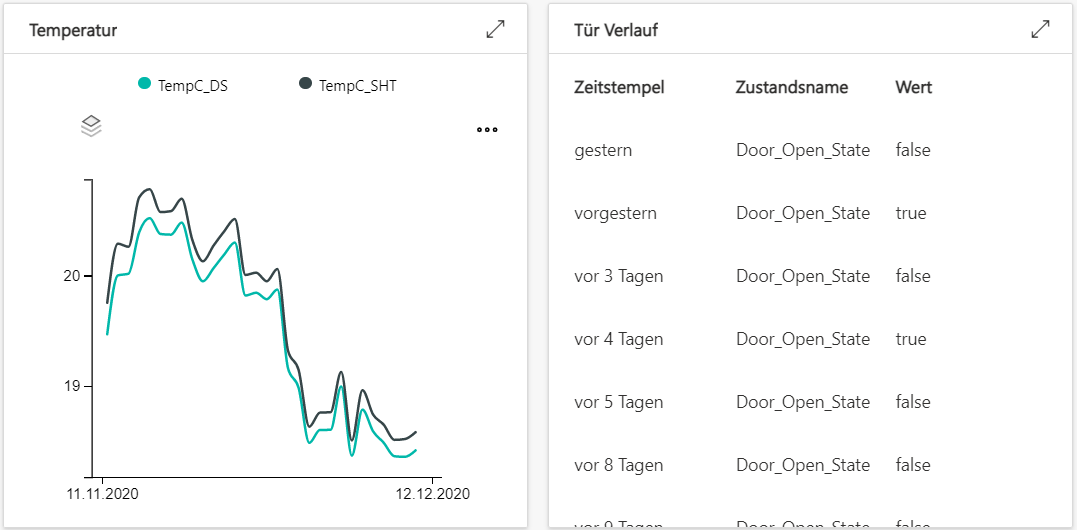
\includegraphics[width=1.0\textwidth]{./images/iotcentral-dashboard.png}  
    \end{center}
  \vspace{-5pt}
  \caption[IoT Central Dashboard]{IoT Central Dashboard}
  \label{fig:iotcentral-dashboard}
  \vspace{-10pt}
\end{figure}

Es gilt hier jedoch zu erwähnen, dass die Möglichkeiten zur Datenvisualisierung zum heutigen Stand noch sehr limitiert und häufig nur wenig konfigurierbar sind. In Abbildung \ref{fig:iotcentral-dashboard} ist beispielsweise zu erkennen, dass die Temperaturdaten anschaulich visualisiert sind, während der Zustand des Türsensors lediglich in einer Tabelle dargestellt wird. Für einfache Szenarien, vor allem dann, wenn die Visualisierung keine große Anforderung ist, reichen die existierenden Möglichkeiten jedoch völlig aus. Neben den Anzeigen eines Dashboards können außerdem Daten auch sehr detailliert über den Analyse-Tab eingesehen werden. Auch Langzeitentwicklungen oder Extremwerte sind hier leicht festzustellen.


Die wohl positivste Überraschung der IoT Central Anwendung war die sehr nützliche Anbindung an die gesamte Microsoft-Infrastruktur. Dies fiel erstmals bei der Einrichtung von Alerts bei Überschreitungen von festgelegten Temperatur- und Luftfeuchtigkeitslimits von festgelegten Limits auf. In IoT Central können nicht nur diese Regeln, sondern auch unzählige Aktionen wie zum Beispiel der Versand einer dynamisch gefüllten E-Mail oder das Aufrufen eines Webhooks konfiguriert werden. Auch das Exportieren von Daten in Azure Blob Storages zur permanenten Datenspeicherung oder Azure Event Hubs für Event Processing und vieles mehr ist mit IoT Central unkompliziert möglich. IoT Central speichert Daten selbst nur 30 Tage lang in einer Time-Series-Datenbank, weswegen ein solcher Export für Szenarien mit Bedarf an Langzeitspeicherung der Daten essentiell wichtig ist. Durch das Exportieren der Daten in die Azure Infrastruktur können nun eine Vielzahl an zusätzlichen Services, wie beispielsweise PowerBI zur besseren Datenvisualisierung, genutzt werden. Auch die Nutzerverwaltung ist direkt an Microsoft gekoppelt. Somit können Zugriffsrechte an Microsoft-Accounts verteilt werden, was gerade in Situationen, in denen bereits eine oft firmeninterne Microsoft-Infrastruktur besteht, sehr hilfreich ist.

\subsection{Architekturübersicht}
\label{sec:Prot:architektur1}

Nachdem nun alle Hardware- und Softwarekomponenten im System sind, hilft es sich einen Überblick über die bisherige Architektur zu schaffen.

\begin{figure}[H]
  \vspace{10pt}
  \begin{center}
    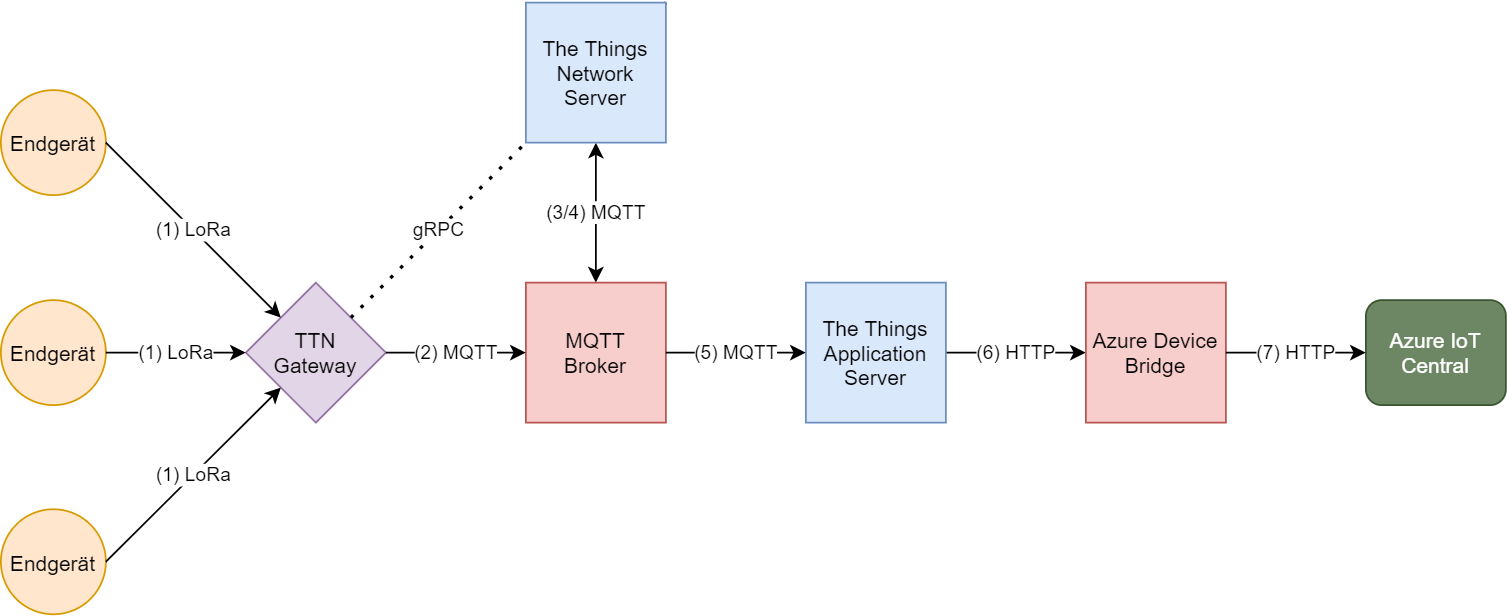
\includegraphics[width=1\textwidth]{./images/ttn-architecture.png}
  \end{center}
  \vspace{-5pt}
  \caption[Prototyp 1: Architekturübersicht]{Prototyp 1: Architekturübersicht}
  \label{fig:ttn_prototype_architecture}
  \vspace{-10pt}
\end{figure}

In Abbildung \ref{fig:ttn_prototype_architecture} ist der Datenfluss einer Uplink-Nachricht eines Endgeräts mit den jeweils genutzten Protokollen durchnummeriert. Es gilt hier zu erwähnen, dass in der Abbildung aus Gründen der Übersichtlichkeit nur Netzwerkkomponenten, die direkt am Datenversand beteiligt sind, dargestellt sind. Dieser beginnt mit dem Datenversand des Endgeräts zum The Things Gateway über LoRa. Empfangen mehrere Gateways im Netzwerk die Nachricht, werden Duplikate später im Network Server gefiltert und können hier somit ignoriert werden. Das Gateway kann durch die Nutzung des Gateway Connector Protocols wahlweise über gRPC Nachrichten direkt an den Network Server oder via MQTT über den Message Broker senden. Erreicht den Network Server eine Nachricht, arbeitet dieser seine Aufgaben ab, wie beispielsweise das Filtern von Duplikaten oder das Validieren der Nachricht. Anschließend leitet der Network Server erneut über den MQTT Broker die nun verarbeitete Nachricht an den Application Server weiter. Dieser ist die letzte Komponente im LoRaWAN-Stack und leitet die Daten über die HTTP Integration an die Azure Device Bridge weiter. Diese Device Bridge, die intern eine Azure Function darstellt, speist diese Daten nun über das HTTP-Protokoll in Azure IoT Central ein. 

\subsection{Evaluation}
\label{sec:Prot:procontra1}

Der erste Prototyp fällt durch einige Stärken sehr positiv auf. Gerade in kleinen Projekten ist die Nutzung des The Things Network ein großer Vorteil, sofern man sich in Reichweite eines öffentlichen Gateways befindet. Da die Kosten für ein eigenes Gateway dadurch wegfallen und lediglich die Endgeräte finanziert werden müssen, handelt es sich hier um eine der günstigsten Möglichkeiten ein LPWA-Netzwerk aufzubauen. Hier gilt es zu erwähnen, dass es keinerlei Garantie gibt, dass ein fremdes Gateway konstant aktiv bleibt, und somit spontane Ausfälle des Netzwerks möglich sind. Ist eine solche Garantie erwünscht, muss also trotz des öffentlichen Netzwerks ein eigenes Gateway eingerichtet werden. Ist ein großes Netzwerk angestrebt, steht neben der Community des The Things Network das Unternehmen The Things Industries für Consulting und fertige Lösungen zur Verfügung, was ebenfalls einen großen Vorteil darstellt. Auch die genutzten Softwarekomponenten bieten einige hilfreiche Features. Sowohl das The Things Network als auch Azure IoT Central Anwendungen sind ausreichend skalierbar und somit für jede Netzwerkgröße geeignet. Speziell Azure IoT Central als IoT Plattform überzeugt durch eine Vielzahl nützlicher Eigenschaften. Besonders hilfreich ist das semantische Mapping von Daten auf Gerätevorlage, wodurch Nutzer keinerlei Wissen über die Datenstruktur benötigen. Außerdem ist IoT Central sehr tief in die Microsoft Infrastruktur eingebettet und erlaubt eine Anbindung der IoT Plattform an unzählige Features wie E-Mail-Alerting, Stream Analytics (Analyse von Echtzeitdaten) oder Langzeitspeicherung. 

In der Umsetzung und Nutzung des Prototypen sind jedoch auch viele Nachteile aufgefallen. Der wohl offensichtlichste dieser Nachteile ist, dass durch die Nutzung von Microsoft Azure Services, und bei großen Deployments auch beim The Things Network, Kosten entstehen. In diesem Kapitel soll jedoch der Fokus auf dem Netzwerk selbst bleiben. Das The Things Network limitiert die Sendezeit aller Geräte strenger als die meisten lokalen Regulierungen durch den Duty Cycle dies tun. So werden jedem Gerät lediglich 30 Sekunden Uplinkzeit und 10 Nachrichten Downlink pro Tag zugeteilt. Nimmt man beispielsweise an, dass eine Nachricht im Schnitt 100 Millisekunden Airtime benötigt, können somit nur 300 Nachrichten pro Tag pro Gerät gesendet werden. Zwar ist dies für viele IoT-Lösungen ausreichend, stellt jedoch eine deutliche Einschränkung gegenüber anderen Techniken dar. Im Prototypen beispielsweise sendet der Temperatur- und Luftfeuchtigkeitssensor alle 20 Minuten eine Nachricht also 72 am Tag und ist somit nicht von der Einschränkung betroffen. \\
Eine sehr unangenehme Eigenschaft des The Things Network ist außerdem, dass bis zum aktuellen Zeitpunkt pro Applikation nur eine Decoder-Funktion erstellt werden kann. Erstellt man also beispielsweise eine Appli\-kation für Temperaturdaten, können nur Geräte mit der gleichen Datenstruktur genutzt werden. Existieren verschiedene Sensortypen müssen also mehrere Applikationen für den eigentlich gleichen Zweck erstellt werden, was sehr schnell sehr unübersichtlich werden kann. Außerdem ist der externe Zugriff auf die Daten sehr umständlich. Zwar veröffentlicht der Application Server die Daten über einen MQTT Broker, jedoch müssen sich Consumer hier pro Application mit verschiedenen Zugangsdaten authentifizieren, was oft nicht praktikabel ist. Um dies zu umgehen, können Integrations, wie in diesem Fall die HTTP-Integration genutzt werden, jedoch muss diese ebenfalls pro Applikation erstellt werden, was erneut eine Fehlerquelle darstellt und bei Änderung der Ziel-URL aufwendig manuell geändert werden muss.\\
Auch die Azure Device Bridge ist ein großer Nachteil dieses Prototypen: der Verwalter des Netzwerks benötigt Softwareentwicklungs- und Azure-Kenntnisse um die Device Bridge aufzusetzen und warten zu können. Auch Azure IoT Central kommt nicht ganz ohne Nachteile aus. So sind die Visualisierungsmöglichkeiten innerhalb der Anwendung sehr gering und zwingen den Nutzer für anschaulichere Dashboards externe Tools wie Microsoft PowerBI zu nutzen, was deutlich mehr Setup erfordert. Außerdem zwingt das semantische Mapping auf Gerätevorlagen den Nutzer gewisse Datentypen zu nutzen. So überträgt der im Prototypen verwendete Sensor die Temperatur und Luftfeuchtigkeit als String, um die Messgenauigkeit beizubehalten, Gerätevorlagen in IoT Central können diese Werte jedoch nur als Zahl interpre\-tieren. Um dies zu umgehen, muss die mitgelieferte Decoder-Function verändert werden und den Wert in einen anderen Datentypen umwandeln. Da bisher keine einheitlichen Normen für Datenformate von IoT-Daten existieren und somit jeder Hersteller ein eigenes Format nutzt, kann dies schnell zu Problemen führen. Außerdem ist der gesamte Softwarestack eine Art Blackbox, da keinerlei Zugriff auf Logs möglich ist. Somit ist es schwer Fehlerquellen im System zu finden. Es gilt auch zu erwähnen, dass dieser Prototyp nur mit Internetzugriff funktioniert, also keine IoT-Netze in einem lokalen Intranet möglich sind.

Allgemein gilt es gerade beim The Things Network hervorzuheben, dass es sich hier weniger um ein fertiges Produkt sondern um die Vision, ein globales, öffentliches LPWA-Netzwerk aufzubauen, handelt. Für fehlende oder noch nicht perfekte Features werden ständig neue Updates veröffentlicht, wodurch das The Things Network in der Zukunft eine potenzielle Lösung für LoRaWAN-Netzwerke jeder Art darstellt. Die Evaluation bewertet lediglich den aktuell Stand des The Things Network für IoT-Lösungen.

\newpage

\section{Prototyp 2: ChirpStack mit InfluxDB und Grafana}
\label{sec:Prot:version2}

Der zweite Prototyp wurde im Vergleich zum ersten ausschließlich mit Open-Source-Software aufgesetzt und nutzt neben einer Azure VM für das Hosting der Anwendung keine externen Services. In diesem Kapitel werden vorerst Erwartungen an den Prototypen gestellt. Anschließend wird eine Alternative zum The Things Network und weitere Software zur Datenverwaltung vorgestellt. Darauf folgen wie beim ersten Prototypen die Umsetzung, Architektur und eine Evaluation des Ergebnisses. In diesem Prototypen werden die Open-Source-Anwendungen \Fachbegriff{ChirpStack} als LoRaWAN-Stack, InfluxDB als Datenbank und Grafana zur Datenvisualisierung verwendet. 

\subsection{Erwartungen}
\label{sec:Prot:erwartungen2}

Da der Aufbau dieses Prototypen keinerlei extern angebotene Services nutzt, kann davon ausgegangen werden, dass das Aufsetzen hier aufwendiger und komplexer ist als beim ersten Prototypen. So müssen unter anderem eigene Server aufgesetzt, konfiguriert und gewartet werden. Hier sind auch Zugriffsrechte und allgemeine Sicherheit vor Angriffen ein großes Thema, welches unter keinen Umständen vernachlässigt werden sollte. Auch das Inbetriebnehmen des eigenen LoRaWAN-Stacks stellt einen erhöhten Aufwand dar, da diese Arbeit im ersten Prototypen durch die Nutzung des The Things Network komplett weggefallen ist. Außerdem muss neben den Endgeräten aufgrund des eigenen privaten LoRaWAN-Netzwerks zwangsweise ein eigenes Gateway gekauft werden. Es wird davon ausgegangen, dass sich lediglich an den Duty Cycle, nicht aber an spezielle Regelungen wie die Fair Use Policy des The Things Network, gehalten werden muss und somit eine höhere Nachrichtenanzahl pro Gerät pro Tag möglich ist. Da vollständige Kontrolle über die Datenbank gegeben ist, wird davon ausgegangen, dass das Festlegen einer für den eigenen Usecase geeigneten Datenstruktur möglich ist. Durch die Nutzung von Grafana wird erwartet, eine Vielzahl an Visualisierungsmöglichkeiten nutzen zu können und alle erwünschten Darstellungen aufbauen zu können. Allgemein wird damit gerechnet, durch das eigene Hosting der Services volle Kontrolle und vor allem Überblick durch Logs über das System zu haben und somit beispielsweise Fehler einfach finden und beheben zu können. Außerdem wird davon ausgegangen, dass dieser Prototyp auch offline in einem Intranet funktionieren könnte.

\subsection{Systemkomponenten}
\label{sec:Prot:systemkomponenten2}

Im Aufbau dieses Prototypen werden eine Vielzahl neuer Softwarekomponenten genutzt, die in diesem Kapitel vorgestellt werden. Es handelt sich bei jeder dieser Komponenten um Open-Source-Anwendungen, die völlig kostenlos genutzt werden können.

\subsubsection{ChirpStack} % Highlights und Architektur aus Doku

Die wohl wichtigste der Komponenten für den Prototypen ist der \Fachbegriff{ChirpStack}. Hierbei handelt es sich um einen LoRaWAN-Stack mit allen in Kapitel \ref{sec:ThHi:architektur} genannten Bauteilen, wobei der Join Server mit in den Application Server integriert ist. Die Funktionen des ChirpStack ähneln denen des The Things Network sehr stark und unterscheiden sich meist nur in Quality-of-Life-Änderungen. Neben dem einzelnen Deployment der Gateway Bridge, des Network Servers und des Application Servers ist außerdem ein Operating System (OS) verfügbar. Das linuxbasierte OS erleichtert die Inbetriebnahme eines LoRaWAN-Stacks stark, indem ein Großteil der Konfigurationsarbeit wegfällt. Da dieser Prototyp aber in einer Azure VM bereitgestellt werden sollte, wurden die einzelnen Komponenenten hier bevorzugt.

\begin{figure}[H]
  \vspace{10pt}
  \begin{center}
    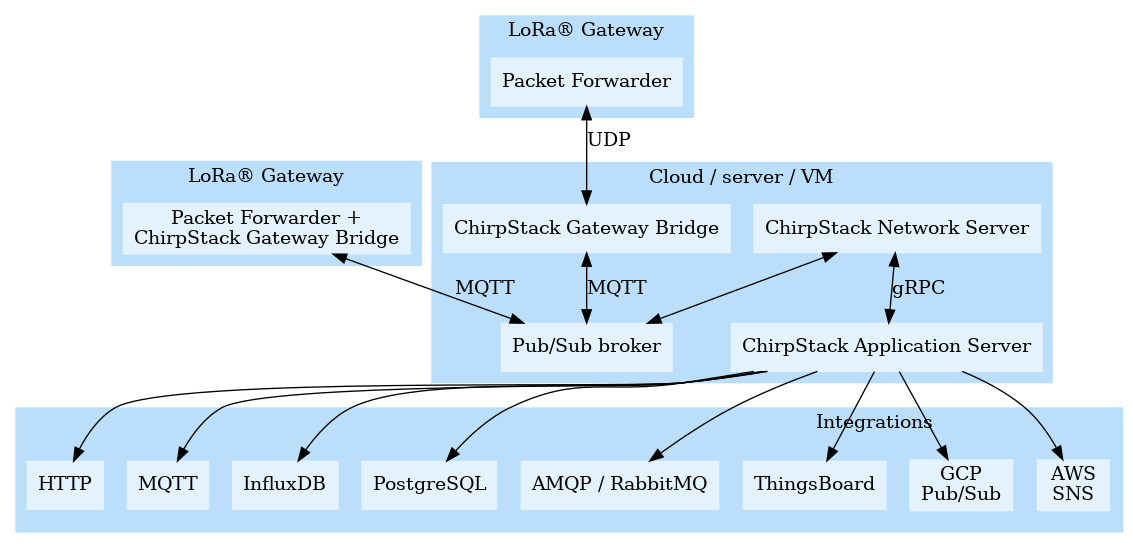
\includegraphics[width=1\textwidth]{./images/chirpstack_architecture.png}
  \end{center}
  \vspace{-5pt}
  \caption[ChirpStack Architektur]{ChirpStack Architektur}
  \caption*{Quelle: {chirpstack.io/static/img/graphs/architecture.dot.png}}
  \label{fig:chirpstack_architecture}
  \vspace{-10pt}
\end{figure}

Wie aus Abbildung \ref{fig:chirpstack_architecture} hervorgeht, ist die Architektur des ChirpStack der des The Things Network sehr ähnlich. Im Zentrum steht ein Pub-Sub-Message-Broker, im Speziellen ein MQTT Broker. Gateways, die nur den Packet Forwarder installiert haben, senden per UDP Nachrichten an die Gateway Bridge, während Gateways, die diese Komponente bereits installiert haben, Nachrichten direkt an den MQTT Broker weiterleiten. Die Gateway Bridge wandelt das LoRa-Datenformat in JSON oder Protobuf um, da dies die vom ChirpStack genutzten Formate zur Weiterverarbeitung sind. Über den Message Broker wandern die Daten weiter in den Network Server. Nachdem dieser seine Aufgaben abgearbeitet hat, sendet der Network Server die Daten weiter an den Application Server. Dies geschieht nicht wie beim The Things Network über den Message Broker, sondern über einen gRPC-Call. Im Application Server können nun wie beim The Things Network Integrations genutzt werden, um die Daten extern erreichbar zu machen \Zitat{ChirpArch.2020}.

\subsubsection{MQTT Consumer} % Erklärung zu TICK bzw TIG#
\label{sec:Prot:systemkomponenten2:mqttcons}
Um Daten vom ChirpStack in eine externe Datenbank zu bewegen, gibt es im Allgemeinen zwei Herangehensweisen. Zum einen können ähnlich zum The Things Network diverse Integrations genutzt werden, die Daten direkt in ein kompatibles Ziel wie beispielsweise HTTP-Endpoints schreiben. Da in diesem Prototypen eine InfluxDB als Datenbank verwendet wird, eignet sich hierfür die InfluxDB-Integration. Diese erfordert kaum Setup und kann Daten in eine beliebige, vom ChirpStack Application Server erreichbare, InfluxDB-Instanz schreiben. Mit dieser Methode macht sich jedoch schnell ein Problem bemerkbar. In der aktuellen ChirpStack-Version ist es nicht möglich, eine eigene Datenstruktur vorzugeben. Durch die relativ unstrukturierte vorgegebene Speicherung wird es später vor allem für Nutzer, die die Daten nicht genau kennen, sehr schwer, diese sinnvoll zu nutzen. Aus diesem Grund wurde ein eigenes Tool\footnote{\url{r-n-d.informatik.hs-augsburg.de:8080/loisbois/mqtt\_lorawan\_consumer}} in der Programmiersprache Go geschrieben, welches die Tatsache nutzt, dass der Application Server Daten stets über die MQTT-Integration an den Message Broker weiterleitet und diese somit über MQTT zugänglich macht. Dieses Tool ist ein MQTT Client mit der Aufgabe, Daten aus dem ChirpStack zu empfangen, diese strukturiert umzuformen und anschließend in das InfluxDB-Line-Protocol, welches im nächsten Kapitel \ref{sec:Prot:systemkomponenten2:influx} weiter erklärt wird, zu übersetzen. 

Über eine Konfigurationsdatei können neben Datenquelle und -ziel die Werte, die verwendet werden sollen, hinterlegt werden. Dies ist besonders wichtig, da es im LoRaWAN-Bereich hierfür erneut keine einheitliche Benennung gibt. So werden Messdaten (also das entschlüsselte LoRaWAN-Payload) im The Things Network unter dem Key ``payload\_fields'' gespeichert, während der ChirpStack den Key ``object'' für diesen Zweck verwendet. Ist in der Konfigurationsdatei eine InfluxDB-Instanz konfiguriert, schreibt das Tool die umgewandelten Daten über die HTTP-Schnittstelle der InfluxDB in den Speicher. Gibt man in der Konfiguration als MQTT-Topic ``application/+/device/+/event/up'' an, wobei das Plus-Zeichen jeweils eine sogenannte Wildcard, also einen beliebigen Wert, darstellt, empfängt der MQTT Consumer die Daten aller registrierten Endgeräte.

Dadurch dass die Programmiersprache Go genutzt wurde kann das Tool zu einer ausführbaren Binary-Datei kompiliert werden. Um diese noch vollständig system\-unabhängig zu machen, also nicht pro Endgerät neu kompilieren zu müssen, wurde außerdem ein eigenes Docker Image erstellt. Da das Docker Image lediglich eine Binary-Datei ausführen muss, und somit keinerlei Systemdateien benötigt, ist das Image mit einer Größe von unter 10 Megabyte außerdem sehr schlank.


\subsubsection{InfluxDB}
\label{sec:Prot:systemkomponenten2:influx}

In Kapitel \ref{sec:Prot:timeseriesdb} wurde bereits erwähnt, dass Time-Series-Datenbanken im IoT-Umfeld immer beliebter werden. In diesem Kapitel wird InfluxDB, eine der verbreitetsten dieser Datenbanken, behandelt.

InfluxDB ist eine, in der Programmiersprache Go entwickelte, Open-Source Time-Series-Datenbank der Firma InfluxData. Die Datenbank wurde im Vergleich zu einer Vielzahl ähnlicher Datenbanken seit Beginn der Enwicklung als Time-Series-DB geplant und dafür optimiert. Die DB unterstützt alle typischen Time-Series-Funktionen wie das Löschen alter Daten oder die Zusammenfassung von Daten in bestimmten Zeiträumen und überzeugt durch Einfachheit, aber auch durch ihre Leichtgewichtigkeit. So können selbst ressourcenarme Geräte wie ein Raspberry Pi hunderte von Sensoren, welche gleichzeitig in eine Datenbank auf dem Einplatinencomputer schreiben, unterstützen \Zitat{TimeSeriesWater.2019}. 

\begin{figure}[H]
  \vspace{10pt}
  \begin{center}
    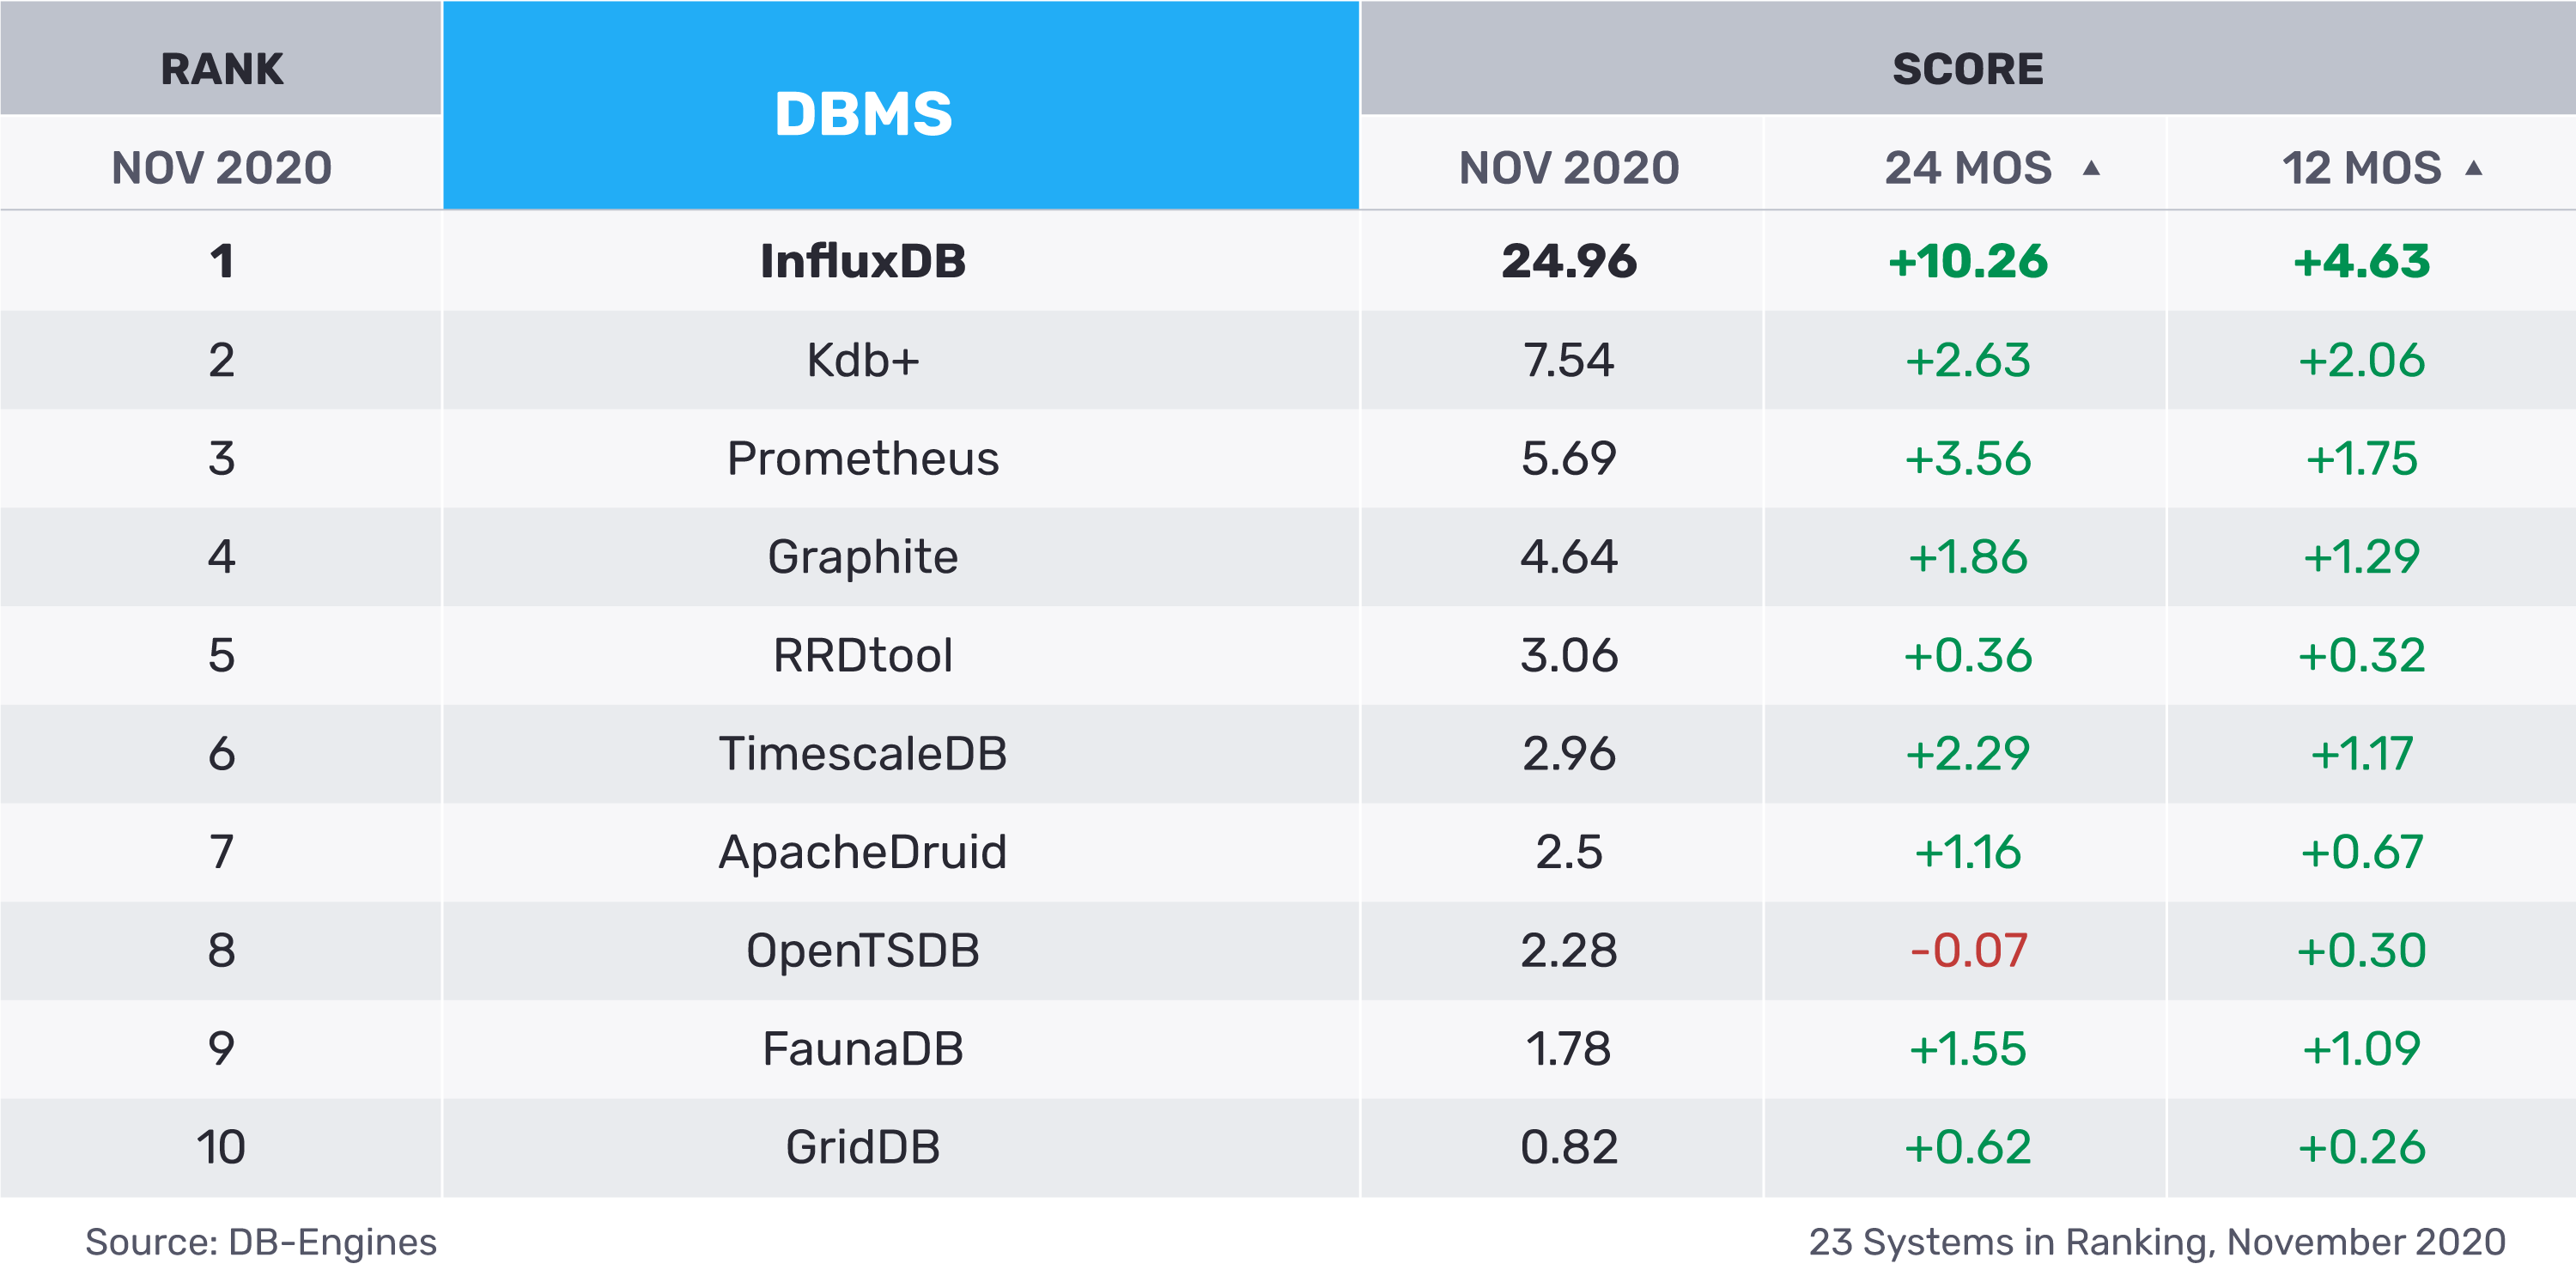
\includegraphics[width=1.0\textwidth]{./images/timeseries_ranking.png}
  \end{center}
  \vspace{-5pt}
  \caption[DB-Engines: Ranking von Time-Series-Datenbanken]{DB-Engines: Ranking von Time-Series-Datenbanken}
  \caption*{Quelle: {influxdata.com/time-series-database}}
  \label{fig:timeseries_ranking}
  \vspace{-10pt}
\end{figure}

InfluxDB wird als beliebteste Time-Series-DB bezeichnet und wird, wie Abbildung \ref{fig:timeseries_ranking} zu entnehmen ist, von unabhängigen Websiten oft mit Abstand auf den ersten Platz im Ranking gesetzt. In den beiden Spalten auf der rechten Seite der Grafik kann die Entwicklung des jeweiligen Scores der letzten 12 und 24 Monate abgelesen werden.

In einer InfluxDB existieren im Allgemeinen drei verschiedene Ressourcen: Nutzer, Retention Policies und Points. Wie in anderen vergleichbaren Datenbanken sind Zugriffs- und Verwaltungsrechte an Nutzer gebunden. Retention Policies bestimmen unter anderem, wie lange die Datenbank Daten speichert, welche Daten zusammengefasst werden können und in welchen Zeitabständen zusammengefasst werden soll. Auch wie Daten zusammengefasst werden kann hier konfiguriert werden, wobei meist der Durchschnitts- oder Maximalwert des Zeitfensters gewählt wird. Abschließend kommt das Kernstück einer jeden Datenbank: die Daten selbst. In einer InfluxDB werden Datenpunkte als \Fachbegriff{Points} bezeichnet.\\
Jeder Point besteht aus einem \Fachbegriff{Measurement}, einem \Fachbegriff{Tagset}, einem \Fachbegriff{Fieldset} und einem \Fachbegriff{Timestamp}. Das Measurement ist dafür da, zusammengehörige Datenpunkte gruppieren zu können. Im Falle des Prototypen wurde die Datenstruktur so gewählt, dass das Measurement den Applikationstyp, zum Beispiel "temp-hum", darstellt. So können alle Temperatur- und Luftfeuchtigkeitsdaten des Systems über das gleiche Measurement gefunden werden. Mit dem Tagset können in einem Key-Value-Format Metainformationen zu dem Point gespeichert werden. Im Prototypen war ein solches Tag der ``deviceName'', der innerhalb eines LoRaWAN-Netzwerks eindeutig ist.\\
Nun kann ein einzelnes Gerät schnell gefunden werden, da zuerst die Auswahl durch das Measurement auf den Applikationstypen reduziert werden kann, und das einzelne Gerät nur noch aus einer stark reduzierten Datenmenge gefiltert werden muss. Die InfluxDB baut außerdem über das Tagset eine Indexstruktur auf, um Lesezugriffe deutlich zu beschleunigen. Im Fieldset finden sich nun die eigentlichen Daten des Points. Auch hier werden Daten in einem Key-Value-Format hinterlegt, jedoch nicht indiziert, da hier primär Schreiboperationen vorgenommen werden. Der letzte Teil des Points ist ein Timestamp, der mit konfigurierbarer Genauigkeit den Zeitpunkt der Aufnahme des Points speichert. 

Points werden in einer InfluxDB durch das Line Protocol serialisiert. Dieses Serialisierungsformat enthält alle vier Komponenten eines Points und beginnt mit dem Namen des Measurements. Nun folgt optional das Tagset. Existieren Tags, werden diese direkt nach dem Measurement mit der Schreibweise ``,key=value'' notiert und aneinandergereiht. Enthält ein Key oder ein Value Leer- oder Sonderzeichen, muss die Zeichenfolge in Anführungszeichen gesetzt werden. Hier gilt es, das führende Komma zu beachten. Ein Leerzeichen beendet das Tagset und beginnt somit das Fieldset welches im gleichen Format wie das Tagset notiert wird, wobei das erste Element auf das führende Komma verzichtet. Hier gilt es zu beachten, dass das Fieldset im Gegensatz zum Tagset nie leer sein darf. Nach einem weiteren Leerzeichen folgt der Timestamp. Ein Point im Line Protocol aus dem Prototypen wird in Abbildung \ref{fig:lineprotocol} gezeigt.

\begin{figure}[H]
  \vspace{10pt}
  \begin{center}
    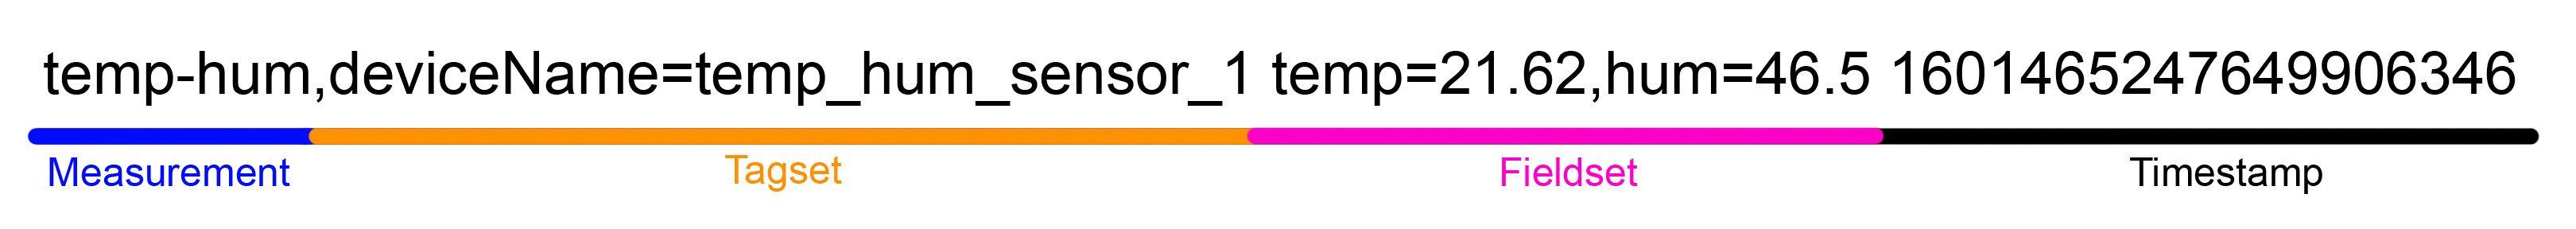
\includegraphics[width=1.0\textwidth]{./images/LineProtocol.jpg}
  \end{center}
  \vspace{-5pt}
  \caption[Datenpunkt im Influx Line Protocol]{Datenpunkt im Influx Line Protocol}
  \label{fig:lineprotocol}
  \vspace{-10pt}
\end{figure}

Das Schreiben von Daten in die InfluxDB funktioniert über einen HTTP Endpoint. Hier können Datenpunkte einzeln oder als Sammlung von Punkten gesendet werden. Erlaubte Formate sind hier entweder JSON oder das Line Protocol, wobei im Prototypen bereits das Line Protocol von der in Kapitel \ref{sec:Prot:systemkomponenten2:mqttcons} erklärten Komponente vorliegt. Beim Verfassen dieses Kapitels wurden die Quellen \cite{TimeSeriesInflux.2020} und \cite{InfluxInternals.2017} genutzt.

 
\subsubsection{Grafana}

Die letzte Softwarekomponente des Prototypen ist Grafana, eine Analyseplattform für Metriken. Mit Grafana können Daten aus verschiedensten Datenquellen wie beispielsweise InfluxDB oder PostgreSQL visualisiert und analysiert werden. Die Open-Source-Plattform zählt zu den beliebtesten Technologien um Dashboards zur Visualisierung von Daten zu erstellen und bietet eine Vielzahl an Möglichkeiten, Daten darzustellen. Reichen die Kernfunktionen nicht aus, kann eine Grafana-Instanz mit unzähligen Plugins erweitert werden. Neben der Datenvisualisierung und -erkundung kann mit Grafana auf Live-Daten reagiert werden. So ist es beispielsweise möglich eine E-Mail an eine festgelegte Adresse zu senden, wenn eine Metrik einen gewissen Wert überschreitet. 

\begin{figure}[H]
  \vspace{10pt}
  \begin{center}
    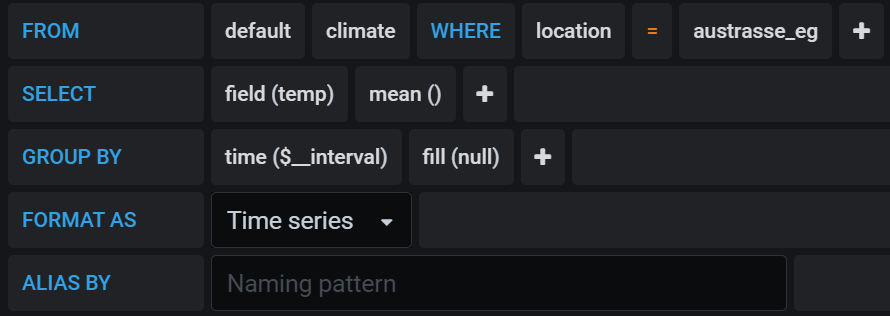
\includegraphics[width=0.85\textwidth]{./images/grafana-sql.png}  
    \end{center}
  \vspace{-5pt}
  \caption[Grafana Query]{Grafana Query}
  \label{fig:grafana-sql}
  \vspace{-10pt}
\end{figure}

Mit Grafana können Visualisierungen durch eine SQL-ähnliche Syntax einfach erstellt werden. Diese Syntax muss jedoch nicht selbst geschrieben werden, sondern kann über einen Wizard zusammengeklickt werden, wie in Abbildung \ref{fig:grafana-sql} erkannt werden kann \Zitat{GrafanaLabs.2020}.

\subsection{Umsetzung}
\label{sec:Prot:umsetzung2}

Im zweiten Prototypen wurde bei der Umsetzung mit der Datenverwaltung und \mbox{-visualisierung} begonnen. Da alle im Prototyp genutzten Komponenten in Docker Containern laufen sollten, jedoch das Orchestrieren einer derart hohen Zahl an Containern sehr aufwendig ist, wurde direkt von Beginn an Docker Compose genutzt, um diesem Problem entgegenzuwirken. Durch die Nutzung von Docker konnte das System lokal im gleichen Environment wie in der Deployment-VM entwickelt und getestet werden. Zu diesem Zeitpunkt war es geplant, den TIG-Stack, bestehend aus \Fachbegriff{Telegraf}, \Fachbegriff{InfluxDB} und \Fachbegriff{Grafana}, für die Datenverwaltung zu nutzen. Telegraf ist hierbei ein Server Agent, der Daten aktiv aus einer Menge von Quellen in eine andere Menge von Zielen schiebt. 

\begin{figure}[H]
  \vspace{10pt}
  \begin{center}
    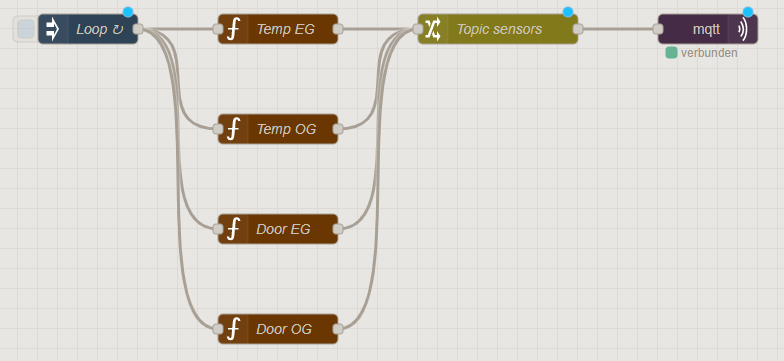
\includegraphics[width=0.75\textwidth]{./images/nodered.png}  
    \end{center}
  \vspace{-5pt}
  \caption[Simulation mit einem NodeRED Flow]{Simulation mit einem NodeRED Flow}
  \label{fig:nodered}
  \vspace{-10pt}
\end{figure}

Um den LoRaWAN-Teil des Prototypen zu simulieren, wurde das grafische Entwicklungswerkzeug \Fachbegriff{NodeRED} genutzt, mit dem in Sekundenschnelle Sensoren, die ihre Daten an einen MQTT Broker senden, durch JavaScript-Funktionen mit Zufallszahlen simuliert werden können. Mithilfe grafischer Bauteile können in NodeRED sogenannte Flows zusammengebaut werden, wie Abbildung \ref{fig:nodered} entnommen werden kann. Der Flow in der Abbildung simuliert zwei Temperatur- und zwei Türsensoren. Nachdem das Tool \Fachbegriff{Telegraf} so konfiguriert wurde, dass Daten aus dem MQTT Broker entnommen und in die InfluxDB geschrieben werden, konnten bereits erste Visualisierungen in Grafana erstellt werden. 

\begin{figure}[H]
  \vspace{10pt}
  \begin{center}
    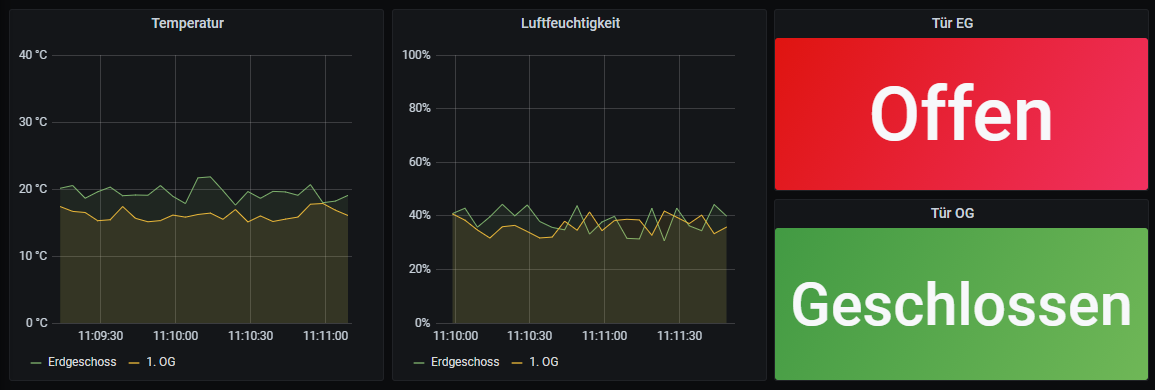
\includegraphics[width=1\textwidth]{./images/simple-dashboard.png}  
    \end{center}
  \vspace{-5pt}
  \caption[Dashboard Simulation]{Dashboard Simulation}
  \label{fig:dashboard-sim}
  \vspace{-10pt}
\end{figure}

In Abbildung \ref{fig:dashboard-sim} ist eine der unzähligen Möglichkeiten zur Datenvisualisierung in Grafana zu sehen. Die dargestellten Daten werden hierbei mit NodeRED zufällig generiert. Zu diesem Zeitpunkt waren fünf Docker Container im Einsatz: Eclipse Mosquitto als MQTT Broker, Telegraf als Data Server Agent, NodeRED zur Simulation des LoRaWAN-Netzes, InfluxDB als Datenbank und Grafana zur Visualisierung.

Nachdem die Speicherung und Visualisierung der Testdaten konfiguriert war, konnte der LoRaWAN-Teil des Prototypen bearbeitet werden. Da alle Komponenten des ChirpStack wie auch alle bisherigen Komponenten in Docker Containern bereitgestellt werden können, wurde so auch auch bei den ChirpStack-Komponenten vorgegangen. Hierfür wurde die offizielle Docker-Compose Vorlage für den ChirpStack\footnote{\url{chirpstack.io/project/guides/docker-compose/}} als Docker-Compose-Deployment genutzt. Da ein Großteil der Konfiguration durch die Vorlage wegfällt, konnte der ChirpStack in Sekundenschnelle gestartet werden. Im ChirpStack Application Server mussten nun neben kleinen Konfigurationsarbeiten, wie der Angabe der IP-Adresse des Network Servers und der Erstellung von Nutzern und deren Rechten, die Geräte, beginnend mit den Gateways, registriert werden. Besonders interessant ist hierbei die sehr ausgereifte Nutzer- und Organisationsverwaltung. Verschiedene Netzwerkbetreiber können sich Gateways teilen und somit ein gemeinsames Netzwerk aufbauen, ohne Zugriff auf die Daten des jeweils anderen zu haben.\\
Dass der ChirpStack richtig aufgesetzt war, konnte mit dem ChirpStack Simulator\footnote{\url{github.com/brocaar/chirpstack-simulator}}, einem Open-Source-Testprogramm für den ChirpStack, getestet werden. Nun konnte die Hardware ins System aufgenommen werden. Das verwendete Gateway verfügte jedoch über keinen freien Speicherplatz, weswegen die Gateway Bridge nicht direkt auf dem Gateway installiert werden konnte, sondern in der Azure VM bereitgestellt werden musste. In der Konfigurationssoftware des Gateways musste nun lediglich die IP-Adresse der Instanz der ChirpStack Gateway Bridge als Ziel für den UDP Packet Forwarder angegeben werden, um die Einrichtung des Gateways abzuschließen. Um die Endgeräte zu registrieren, konnten nun ähnlich wie beim The Things Network in Kapitel \ref{sec:Prot:umsetzung1} Applikationen erstellt werden, die eine Art Container für zusammengehörige Geräte darstellen. Ein elementarer Unterschied fiel im Vergleich zum ersten Prototypen auf: Decoder-Funktionen sind im ChirpStack nicht an die Applikation, sondern an sogenannte Device-Templates gebunden, welche dann wiederum verschiedenen Endgeräten zugeteilt werden. Somit können Geräte mit verschiedenen Datenstrukturen, die jedoch einen ähnlichen Zweck wie beispielsweise Temperaturmessung verfolgen, mit einer Applikation abgedeckt werden. Nachdem für die beiden Sensortypen Device-Templates erstellt waren und die Geräte selbst registriert waren, konnten bereits LoRaWAN-Pakete empfangen werden. 

\begin{figure}[H]
  \vspace{10pt}
  \begin{center}
    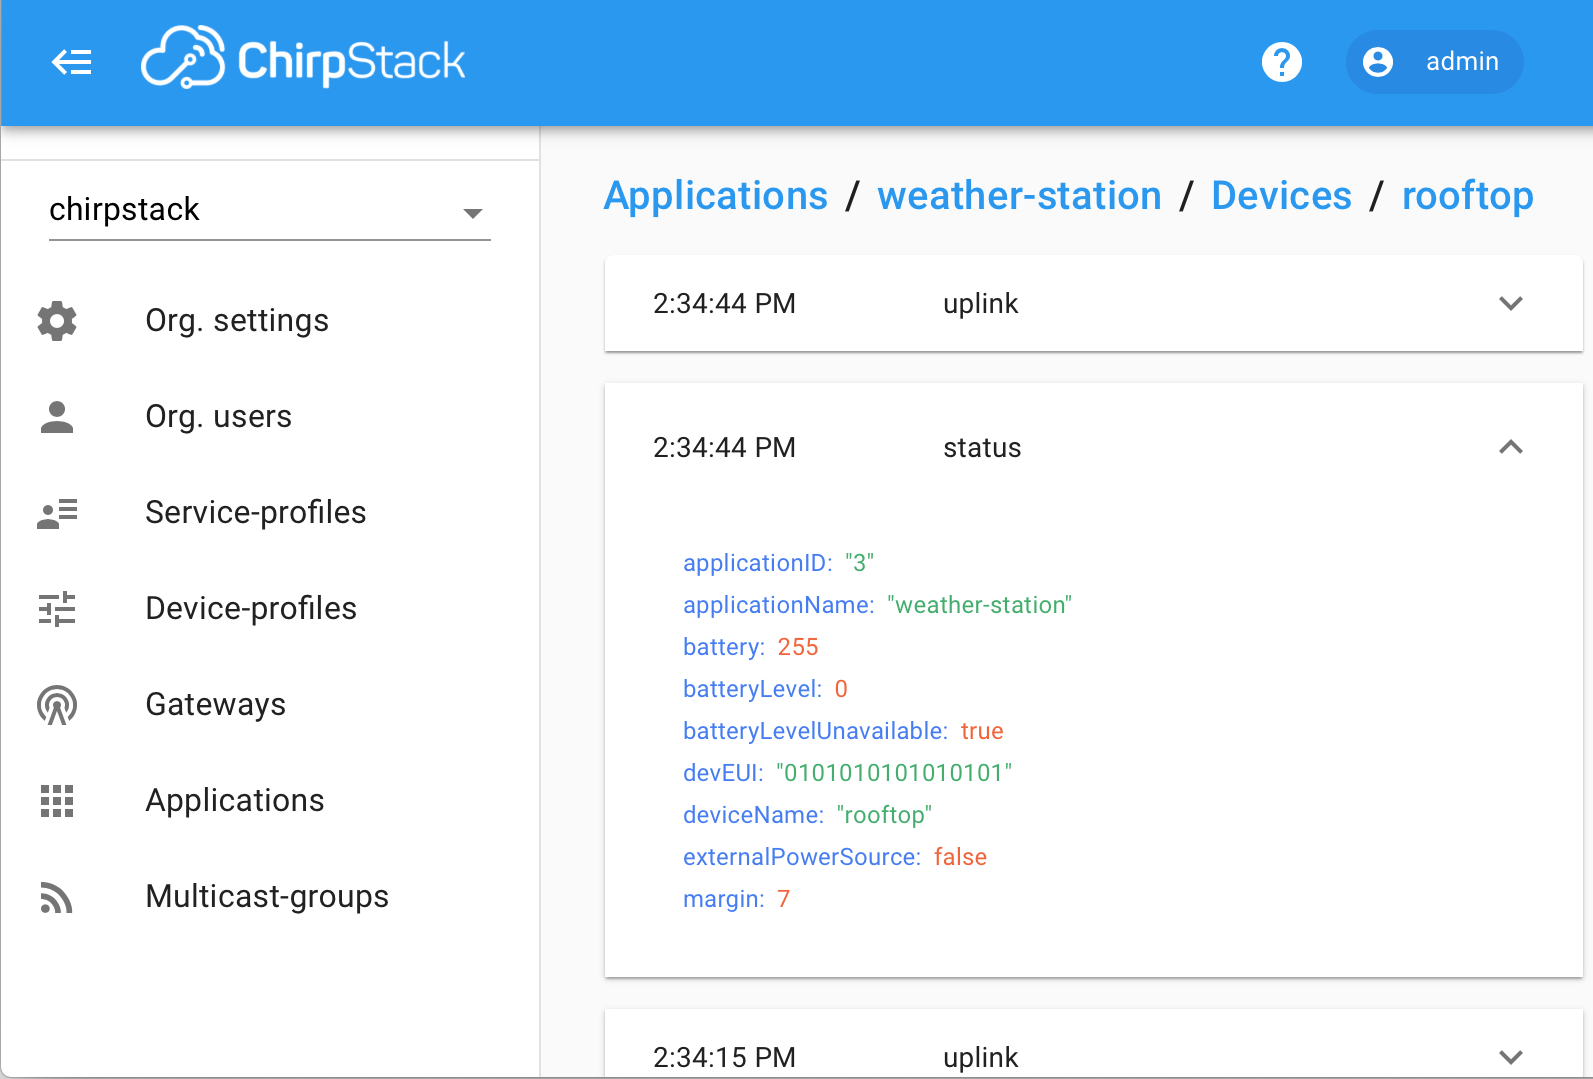
\includegraphics[width=0.9\textwidth]{./images/chirpstack-ui.png}
  \end{center}
  \vspace{-5pt}
  \caption[ChirpStack Benutzeroberfläche]{ChirpStack Benutzeroberfläche}
  \caption*{Quelle: {chirpstack.io/application-server (bearbeitet)}}
  \label{fig:chirpstack-ui}
  \vspace{-10pt}
\end{figure}

Abbildung \ref{fig:chirpstack-ui} zeigt ein Beispiel, wie der Datenempfang eines registrierten und konfigurierten Sensors in der Benutzeroberfläche des ChirpStack Application Servers aussehen könnte. 

Nun war es an der Zeit, den LoRaWAN-Teil des Prototypen mit der Datenverwaltung, in der bisher nur Testdaten gespeichert wurden, zu verbinden. Der erste Versuch fand hierfür mit der InfluxDB-Integration des ChirpStack Application Server statt. Durch die Angabe des HTTP-Write-Endpoints und der Authentifizierungsparameter der InfluxDB konnte die Integration schnell umgesetzt werden. Die Daten von empfangenen LoRaWAN-Paketen wurden nun erfolgreich in die Time-Series-Datenbank geschrieben. Bei der genaueren Betrachtung der gespeicherten Daten fiel jedoch schnell ein großes Problem auf: die InfluxDB-Integration speichert jeden Point (siehe Kapitel \ref{sec:Prot:systemkomponenten2:influx}) mit dem Namen des sendenden Endgeräts und dem Präfix \mbox{``device\_frmpayload\_data''} als Measurementnamen. Da es in der InfluxDB-Integration zum aktuellen Stand nicht möglich ist, eine eigene Datenstruktur zu verwenden, ist man an diese Benennung gebunden. Das Problem: da Points nun mit dem Gerätenamen als Measurement gespeichert werden, verfällt die Gruppierung von Geräten in Applikationen und resultiert in einer schnell sehr unübersichtlich werdenden Datenstruktur. Auch der Versuch den Server Agent \Fachbegriff{Telegraf} mit der MQTT-API, über die der ChirpStack empfangene Daten standardmäßig verbreitet, zu diesem Zweck zu nutzen, führte zum gleichen Problem. Aus diesen Gründen wurde für genau diesen Zweck der bereits erwähnte MQTT Consumer in der Programmiersprache Go entwickelt, dessen Funktionsprinzip bereits in Kapitel \ref{sec:Prot:systemkomponenten2:mqttcons} erläutert wurde. Die Komponente ähnelt also Telegraf stark, wobei der Schritt der Umwandlung des Datenformats hinzukommt. Auch diese Komponente wurde als \mbox{Docker} Container mit ins System aufgenommen und konnte leicht integriert werden. Versucht man nun beispielsweise einen speziellen Temperatursensor zu finden, ist es nicht nötig, alle Geräte zu durchsuchen, da zuerst nach dem Applikationstypen, welcher in der Datenbank das Measurement darstellt, gefiltert werden kann.\\
Somit war nun die Datenstruktur deutlich sinnvoller aufgebaut als die Datenstruktur der Integrations zum aktuellen Entwicklungsstand. Das System stand soweit fest und konnte nun auf das Production-System, im Fall dieses Prototypen eine Microsoft Azure VM, geladen werden. Auf dieser VM musste lediglich die Docker-Compose-Konfigurationsdatei genutzt werden, um das gleiche System wie im lokalen Environment herzustellen. Außerdem mussten Ports wie 1883 für MQTT und 80 für HTTP freigegeben werden, um die VM von außen erreichbar zu machen. Um das Gateway ins System aufzunehmen musste lediglich die IP-Adresse der Gateway Bridge in der Gatewaykonfiguration angepasst werden und das System lief vollständig im Production-System.

\begin{figure}[H]
  \begin{center}
    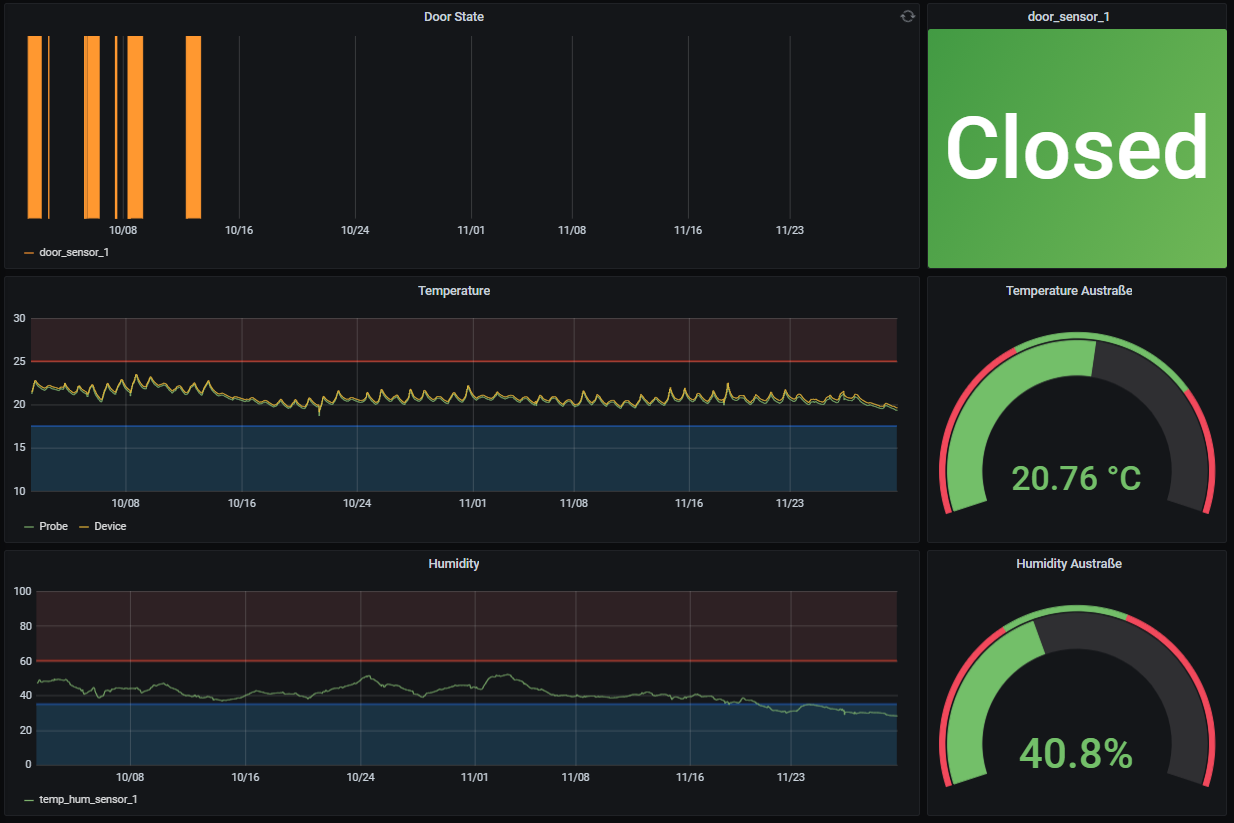
\includegraphics[width=1\textwidth]{./images/dashboard-longterm.png}  
    \end{center}
  \vspace{-5pt}
  \caption[IoT Dashboard: 2 Monate]{IoT Dashboard: 2 Monate}
  \label{fig:dashboard-longterm}
  \vspace{-5pt}
\end{figure}

Mit Grafana konnten nun anschauliche Dashboards über reale IoT-Daten erstellt werden. Abbildung \ref{fig:dashboard-longterm} zeigt das finale IoT-Dashboard und visualisiert die Temperatur und die Luftfeuchtigkeit eines Raumes sowie den Öffnungszustand einer Tür über jeweils einen Zeitraum von zwei Monaten.


\subsection{Architekturübersicht}
\label{sec:Prot:architektur2}

Gerade beim zweiten Prototypen ist es aufgrund der erhöhten Komplexität durch die hohe Anzahl an selbstverwalteten Services sinnvoll, sich einen Überblick über die Netzwerkarchitektur zu verschaffen. 

\begin{figure}[H]
  \vspace{10pt}
  \begin{center}
    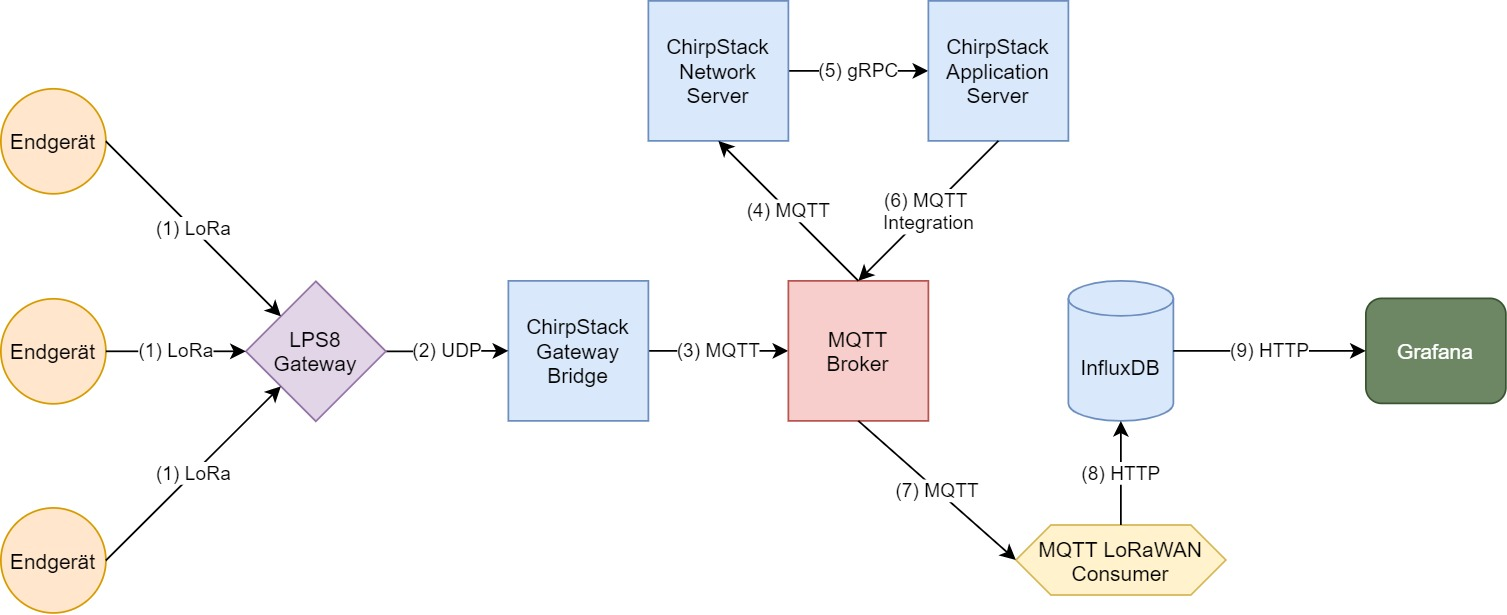
\includegraphics[width=1\textwidth]{./images/chirpstack_prototyp_architecture.jpg}
  \end{center}
  \vspace{-5pt}
  \caption[Prototyp 2: Architekturübersicht]{Prototyp 2: Architekturübersicht}
  \label{fig:chirpstack_prototype_architecture}
  \vspace{-10pt}
\end{figure}

In Abbildung \ref{fig:chirpstack_prototype_architecture} wird der Weg einer Nachricht vom LoRa-Endgerät bis zur Visualisierung in Grafana dargestellt. Nachdem das Gateway eine LoRaWAN-Nachricht von einem Endgerät empfangen hat, wird diese über das UDP Packet Forwarder Protocol an die Gateway Bridge weitergeleitet. Die Gateway Bridge legt diese Nachricht nun im MQTT Broker ab. Hätte das Gateway selbst eine Gateway Bridge installiert, könnte es die Nachricht direkt zum MQTT Broker senden. Der Network Server nimmt die Nachrichten als Subscriber vom MQTT Broker und verarbeitet diese weiter. Anders als beim The Things Network leitet dieser die verarbeiteten Nachrichten via gRPC direkt an den Application Server weiter und geht nicht erneut über den Message Broker. Die standardmäßig aktive MQTT Integration veröffentlicht nun die vom Application Server dekodierten Daten auf dem MQTT Broker. Die Daten verlassen nun den LoRaWAN-Stack, indem der selbst entwickelte MQTT Consumer diese vom Broker liest und über die HTTP-Schnittstelle in die InfluxDB schreibt. Grafana nutzt die Unterstützung für InfluxDB, um direkt aus der Datenbank Daten zur Visualisierung einzulesen. 

\subsection{Evaluation}
\label{sec:Prot:procontra2}

Auch die Evaluation des zweiten Prototypen beginnt mit einem Blick auf die Stärken des Systems, beginnend mit dem LoRaWAN-Teil. Mit dem ChirpStack kann ein eigenes LoRaWAN in kurzer Zeit instand gesetzt werden. Hierbei kann selbst entschieden werden, ob alle Softwarekomponenten online, verteilt oder gar vollständig offline in einem Intranet bereitgestellt werden sollen. Für sehr große Netzwerke besteht hier die Möglichkeit, das System nicht nur vertikal, sondern auch horizontal zu skalieren, indem Komponenten mehrfach gestartet werden, um die Systemlast pro Komponente zu senken. Wird ein LoRaWAN-Netzwerk mit dem ChirpStack aufgesetzt, ist dieses Netzwerk stets ein komplett privates Netzwerk. Dies birgt den Vorteil, dass lediglich die in Kapitel \ref{sec:ThHi:technisch} erwähnten lokalen LoRaWAN-Regulierungen, also der Duty Cycle, eingehalten werden müssen. Auf Netzwerkregulierungen wie eine maximale Uplinkzeit oder eine festgelegte Anzahl von Downlinknachrichten pro Tag beim The Things Network muss hier nicht geachtet werden. Somit ist es in einem privaten Netzwerk möglich, eine deutlich höhere Anzahl an Nachrichten zu senden.\\
Weiter bietet der ChirpStack eine durchdachte Nutzerverwaltung. Neben Nutzer- und Zugriffsrechten können beispielsweise Organisationen erstellt werden, die im Netzwerk koexistieren können, ohne die Daten des anderen zu sehen. So können Nutzergruppen wie beispielsweise verschiedene Abteilungen eines Unternehmens voneinander separiert werden, ohne dafür ein weiteres Netzwerk aufbauen zu müssen. Bei der Planung war die Erwartung, dass das Aufsetzen des Gateway im Netzwerk deutlich aufwendiger ist als beim The Things Network, da dort stets mit der Einfachheit durch den Verkauf eigener, vorkonfigurierter Gateways geworben wird. In der Umsetzung stellte sich dies jedoch als ähnlich einfach heraus und verursachte keinerlei Probleme. Auch das Hinzufügen neuer Endgeräte ähnelt dem The Things Network und funktionierte stets mühelos.\\
Hierbei fiel schnell ein kleiner Aspekt auf, der jedoch einen der größten Vorteile des ChirpStacks darstellt. Durch Device Templates können verschiedene Endgeräte mit unterschiedlichen Datenstrukturen in einer Applikation gruppiert werden, da nun Decoder-Funktionen nicht mehr pro Applikation sondern pro Device Template erstellt werden können. Somit ist es im ChirpStack beispielsweise möglich, Temperatursensoren von verschiedenen Herstellern in der gleichen Applikation zu verwalten, wodurch eine deutlich sinnvollere Datenstruktur entsteht. Auch die standardmäßig aktive MQTT-API für den externen Zugriff auf LoRaWAN-Daten bietet Vorteile gegenüber der des The Things Network. Während es nämlich im TTN nötig war, pro Applikation eigene Credentials für den Datenzugriff zu nutzen und somit pro Applikation eine eigene MQTT-Verbindung aufbauen zu müssen, reicht im ChirpStack eine einzige Verbindung aus. Ist ein MQTT-Client mit dem ChirpStack verbunden, kann er durch das Nutzen von Wildcards eine Subscription für alle Applikationen starten. Allgemein ist der ChirpStack außerdem sehr ausführlich dokumentiert und verfügt über eine große und hilfsbereite Community.\\
Auch die beiden Komponenten in der Datenverwaltung weisen einige Vorteile auf. Die InfluxDB ist eine äußert einfach nutzbare Datenbank. Die Inbetriebnahme ist durch die Nutzung von Docker sehr unkompliziert und erfordert kaum Konfiguration. Die Datenbank benötigt nur sehr geringe Systemressourcen und ist durch Retention Policies deutlich effizienter im Umgang mit Festplattenspeicher als typische relationale Datenbanken. Für große Szenarien existieren hier außerdem verteilte Deployments oder gar Cloudlösungen. Das Highlight des Prototypen ist das Visualisierungstool Grafana. Neben der InfluxDB kann Grafana aus unzähligen Datenquellen selbst gleichzeitig Daten anfordern und anschließend visualisieren oder regelbasiert auf Daten durch den Versand von E-Mails oder viele weitere Kanäle reagieren. Die Visualisierungsmöglichkeiten sind hierbei beinahe endlos. Selbst komplexe Queries an die Datenbank können mit einer SQL-ähnlichen Syntax zusammengeklickt werden und einfach dargestellt werden. Reichen die existierenden Features nicht aus, kann Grafana durch eine Vielzahl an Plugins erweitert werden. Da alle Komponenten typischerweise in Docker Containern gestartet werden, kann das System einerseits einfach lokal getestet, aber andererseits auch unkompliziert auf ein Production-System geladen werden. Durch die eigene Serververwaltung steht dem Netzbetreiber der Zugriff auf Logs und somit die Möglichkeit zur Fehlersuche und -behebung zur Verfügung. Außerdem kann das System durch das vorsichtige Freischalten von Ports zur Außenwelt von einem Großteil möglicher Angriffe geschützt werden. Im hier aufgesetzten Prototypen kann auf den ChirpStack Application Server beispielsweise nur aus dem eigenen Netzwerk zugegriffen werden. Letztendlich kann als Vorteil notiert werden, dass alle Netzwerkkomponenten in der gleichen Umgebung, sowohl online als auch offline, bereitgestellt werden können und dadurch die gesamte Verwaltung anders als beim ersten Prototypen an einer zentralisierten Stelle stattfindet.

Auch der zweite Prototyp birgt Nachteile. Der wohl offensichtlichste und größte dieser Nachteile ist, dass für die Instandsetzung des Prototypen selbst Server aufgesetzt und verwaltet werden müssen. Auch Sicherheit spielt hier eine große Rolle, da man Server durch unvorsichtige Konfiguration einer großen Angriffsfläche aussetzt. Soll ein cloudbasiertes System aufgesetzt werden, werden nicht nur grundlegende Kenntnisse in Linux, Docker und Sicherheitskonfiguration, sondern auch Kenntnisse in einer Cloud-Plattform wie beispielsweise Microsoft Azure benötigt. Müssen, wie in dieser Arbeit, weitere Tools wie der eigene MQTT-Consumer selbst implementiert werden, sind außerdem Programmierkenntnisse vonnöten. \newpage
Hand in Hand mit der eigenen Serveraufsetzung geht ein weiterer großer Nachteil dieses Prototypen: das System benötigt eine eigene Backupstrategie. Mit der hier gezeigten Architektur speichert das System jegliche Daten im Dateisystem. Gehen diese Daten verloren, gibt es ohne eine Backuplösung keine Möglichkeit, die verlorenen Daten wiederherzustellen. Neben klassischen Strategien wie dem direkten Speichern von Snapshots im Filesystem ist hier die einfachste Lösung, eine cloudbasierte und extern verwaltete InfluxDB-Instanz statt einer selbst bereitgestellten Instanz zu nutzen. Ein weiterer klarer Nachteil bezieht sich auf das LoRaWAN-Netzwerk selbst. Da das Netzwerk vollständig privat ist, muss die gesamte Abdeckung des zu unterstützenden Gebietes selbst mit eigenen Gateways aufgebaut werden. Gerade für mobile Endgeräte oder Szenarien, in denen Geräte in verschiedenen Regionen platziert sind, ist also die Nutzung des The Things Network und die damit verbundene existierende Netzabdeckung eine bessere Lösung. Auch in kleinen Projekten macht sich dies bemerkbar. Um LoRaWAN-Endgeräte nutzen zu können, muss bei diesem Prototypen zwingend ein eigenes Gateway in Betrieb genommen werden, was die Kosten deutlich vergrößert, während im The Things Network durch die existierende Abdeckung oft nicht zwangsweise ein eigenes Gateway aufgesetzt werden muss. Da fremde Gateways im TTN jedoch stets unerwartet vom Netz genommen werden können, sollte in Szenarien, in denen die Netzwerkstabilität essentiell wichtig ist, jedoch immer ein eigenes Gateway in Betrieb genommen werden. Dies gilt für beide Prototypen und ist somit nicht als Nachteil eines eigenen LoRaWAN-Netzwerks zu werten.\\ 
Ein Feature, welches sich im ersten Prototypen als sehr nützlich erwiesen hat, fehlt im zweiten Prototypen: das semantische Datenmapping. Daten werden hier in einer selbst definierten Struktur in eine Datenbank gespeichert und müssen stets vom Nutzer interpretiert werden. Somit ist die Nutzung der Anwendung für Personen, die die Datenstruktur nicht genau kennen, schwieriger als beim ersten Prototypen. Abschließend muss der Nachteil erwähnt werden, dass es beim zweiten Prototypen an einer Anbindung an ein Netz aus Services wie beim ersten Prototypen an Microsoft mangelt. So müssen hier Funktionen die auf externe Services zugreifen wie beispielsweise E-Mail-Alerts selbst konfiguriert werden, da das Tool selbst an keinen E-Mail-Server angebunden ist. Allgemein ist der zweite Prototyp also sehr gut in der Visualisierung der Daten, muss jedoch um einigen Features des ersten Prototypen nachzukommen, um weitere Konfiguration oder gar neue Softwarekomponenten erweitert werden.

